\documentclass[14pt,a4paper]{extarticle}
\usepackage[utf8]{inputenc}
%koi8-r]{inputenc}
\usepackage[english,russian]{babel}
\usepackage{amsmath}
\usepackage{amsfonts}
\usepackage{amssymb}
\usepackage[usenames,dvipsnames,svgnames,table]{xcolor}

\usepackage[hypcap]{subcaption}

\usepackage{float} % Required for specifying the exact location of a figure or table

\usepackage{placeins}

% \usepackage[backend=bibtex, style=numeric, sorting=none, maxnames=3, minnames=3, hyperref=true, url=false, isbn=false, backref=true]{biblatex}
% \usepackage[backend=bibtex]{biblatex}
% \bibliography{sample}
\usepackage[style=alphabetic, maxnames=5, minnames=5]{biblatex}
\renewcommand*{\bibfont}{\footnotesize}
%  \bibliography{sample}
\addbibresource{mybib.bib}

\usepackage{graphicx} % Required for the inclusion of images
% \usepackage[hypcap]{subcaption}
\usepackage[font=small]{caption}

\usepackage{textcomp}
\usepackage[version=4]{mhchem}
% \usepackage{translator}

\usepackage{tabulary}

% \usepackage{cleveref}
\usepackage[colorlinks=true, linkcolor=Maroon, citecolor=OliveGreen]{hyperref}

% \hyphenation{элек-трон-пози-трон-ны-ми}

\usepackage{setspace}
\onehalfspacing

\usepackage{commath}

% \newcommand{\fref}[1]{Рис.~\ref{#1}}
% \newcommand{\tref}[1]{Таб.~\ref{#1}}
% \newcommand{\eref}[1]{(\ref{#1})}

\newcommand*\rot{\rotatebox{90}}

\usepackage[separate-uncertainty = true, multi-part-units=single,
range-phrase=\text{\,--\,}, range-units=single,
per-mode = symbol]{siunitx}
\DeclareSIUnit\lr{\textup{л}}
\DeclareSIUnit\Par{\textup{Па}}
\DeclareSIUnit\kPar{\textup{кПа}}
\DeclareSIUnit\MPar{\textup{МПа}}

\DeclareSIUnit\nmr{\textup{нм}}
\DeclareSIUnit\umr{\textup{$\mu$м}}
\DeclareSIUnit\mmr{\textup{мм}}
\DeclareSIUnit\cmr{\textup{см}}
\DeclareSIUnit\mr{\textup{м}}
\DeclareSIUnit\kmr{\textup{км}}
\DeclareSIUnit\sr{\textup{с}}
\DeclareSIUnit\msr{\textup{мс}}

\DeclareSIUnit\nsr{\textup{нс}}
\DeclareSIUnit\Xrad{\textup{X$_{0}$}}
\DeclareSIUnit\mgr{\textup{мг}}
\DeclareSIUnit\gr{\textup{г}}
\DeclareSIUnit\kgr{\textup{кг}}


%  Углы
\DeclareSIUnit\radianru{\textup{рад}}
\DeclareSIUnit\mradianru{\textup{мрад}}

%  Частота
\DeclareSIUnit\uHzr{\textup{$\mu$Гц}}
\DeclareSIUnit\mHzr{\textup{мГц}}
\DeclareSIUnit\Hzr{\textup{Гц}}
\DeclareSIUnit\kHzr{\textup{кГц}}
\DeclareSIUnit\MHzr{\textup{МГц}}
\DeclareSIUnit\GHzr{\textup{ГГц}}

\DeclareSIUnit\pbarnr{\textup{пб}}
\DeclareSIUnit\nbarnr{\textup{нб}}
\DeclareSIUnit\barnr{б}
\DeclareSIUnit\bear{медведь}
\DeclareSIUnit\mNr{\textup{мН}}
\DeclareSIUnit\Nr{\textup{Н}}
\DeclareSIUnit\kNr{\textup{кН}}
\DeclareSIUnit\dynr{\textup{дин}}
\DeclareSIUnit\mmrtst{\textup{мм.\,рт.\,ст.}}
\DeclareSIUnit\radr{\textup{рад}}

%  Заряд
\DeclareSIUnit\aCr{\textup{аКл}}
\DeclareSIUnit\fCr{\textup{фКл}}
\DeclareSIUnit\pCr{\textup{пКл}}
\DeclareSIUnit\nCr{\textup{нКл}}
\DeclareSIUnit\uCr{\textup{$\mu$Кл}}
\DeclareSIUnit\mCr{\textup{мКл}}
\DeclareSIUnit\Cr{\textup{Кл}}
\DeclareSIUnit\kCr{\textup{кКл}}
\DeclareSIUnit\MCr{\textup{МКл}}

%  Энергия
\DeclareSIUnit\mJr{\textup{мДж}}
\DeclareSIUnit\Jr{\textup{Дж}}
\DeclareSIUnit\kJr{\textup{кДж}}
\DeclareSIUnit\MJr{\textup{МДж}}
\DeclareSIUnit\eVr{\textup{эВ}}
\DeclareSIUnit\keVr{\textup{кэВ}}
\DeclareSIUnit\MeVr{\textup{МэВ}}
\DeclareSIUnit\GeVr{\textup{ГэВ}}

%  Ёмкость
\DeclareSIUnit\Fr{\textup{Ф}}
\DeclareSIUnit\mFr{\textup{мФ}}
\DeclareSIUnit\uFr{\textup{$\mu$Ф}}
\DeclareSIUnit\nFr{\textup{нФ}}
\DeclareSIUnit\pFr{\textup{пФ}}
\DeclareSIUnit\fFr{\textup{фФ}}

%  Ток
\DeclareSIUnit\Ar{\textup{А}}
\DeclareSIUnit\mAr{\textup{мА}}
\DeclareSIUnit\uAr{\textup{$\mu$А}}
\DeclareSIUnit\nAr{\textup{нА}}
\DeclareSIUnit\pAr{\textup{пА}}
\DeclareSIUnit\fAr{\textup{фА}}

%  Напряжение
\DeclareSIUnit\uVr{\textup{$\mu$В}}
\DeclareSIUnit\mVr{\textup{мВ}}
\DeclareSIUnit\Vr{\textup{В}}
\DeclareSIUnit\kVr{\textup{кВ}}
\DeclareSIUnit\MVr{\textup{МВ}}
\DeclareSIUnit\GVr{\textup{ГВ}}

% Время
\DeclareSIUnit\sr{\textup{с}}
\DeclareSIUnit\msr{\textup{мс}}
\DeclareSIUnit\usr{\textup{$\mu$с}}
\DeclareSIUnit\nsr{\textup{нс}}
\DeclareSIUnit\psr{\textup{пс}}

%  Магнитное поле
\DeclareSIUnit\teslaru{\textup{Тл}}
\DeclareSIUnit\mteslaru{\textup{мТл}}
\DeclareSIUnit\gaussru{\textup{Гс}}
\DeclareSIUnit\kgaussru{\textup{кГс}}
\DeclareSIUnit\Maussru{\textup{МГс}}
\DeclareSIUnit\Gaussru{\textup{ГГс}}

\DeclareSIUnit\clight{\text{\ensuremath{c}}}

\renewcommand{\labelenumii}{\arabic{enumii}.}

% \topmargin -20 mm
% \oddsidemargin 5 mm
% \textheight 250 mm
% \textwidth 160 mm


\usepackage[height=25cm, a4paper, hmargin={25mm, 10mm}, vmargin={2cm, 2cm}]{geometry}


\usepackage{tikz}
\usetikzlibrary{arrows, shapes, chains}
\usepackage[compat=1.1.0]{tikz-feynman}



\title{Отчёт по научно исследовательской--практике}% Title

\author{Георгий Павлович \textsc{Разуваев}\\{\smallаспирант 3-го года обучения ИЯФ им. Г.\,И.\,Будкера, СО РАН}} % Author name
% \author{}

\date{26 января 2017\,г.} % Date for the report

\begin{document}

% \maketitle % Insert the title, author and date

%%%%%%%%%%%%%%%%%%%%%%%%%%%%%%%%%%%%%%%%%%%%%%%%%%%%%%%%%%%%%%%%%%%%%%%%
\begin{titlepage}

\begin{center}

Федеральное Агентство Научных Организаций

\vspace{.5cm}

ФЕДЕРАЛЬНОЕ ГОСУДАРСТВЕННОЕ БЮДЖЕТНОЕ УЧРЕЖДЕНИЕ НАУКИ \\
ИНСТИТУТ ЯДЕРНОЙ ФИЗИКИ ИМ. Г.\,И.~БУДКЕРА \\
СИБИРСКОГО ОТДЕЛЕНИЯ РОССИЙСКОЙ АКАДЕМИИ НАУК

\vspace{2cm}

ОТЧЁТ \\
О НАУЧНО-ИССЛЕДОВАТЕЛЬСКОЙ РАБОТЕ \\
ЗА VII СЕМЕСТР ОБУЧЕНИЯ В АСПИРАНТУРЕ

\vspace{1.5cm}

\boldmath
\textbf{Измерения сечения реакции
$e^+ e^- \to \eta \gamma, \, \pi^0 \gamma \to 3 \gamma$\\
с детектором КМД-3 на коллайдере ВЭПП-2000}
\unboldmath


\end{center}

\vspace{2cm}

\underline{Специальность:} 01.04.16 Физика атомного ядра и элементарных частиц

\vspace{.5cm}

\underline{Тема научных исследований в аспирантуре:} Изучения реакции $e^+ e^- \to \eta \gamma, \, \pi^0 \gamma \to 3 \gamma$ в диапазоне энергий \SIrange{.6}{2.}{\GeVr}

\vspace{2cm}

\begin{minipage}[t]{0.5\textwidth}
\hspace{3cm}
\end{minipage}
\begin{minipage}[t]{0.5\textwidth}
Оценка \underline{\hspace{3cm}}
\end{minipage}


\vspace{1cm}

\begin{minipage}[t]{0.5\textwidth}
Научный руководитель
\end{minipage}
\begin{minipage}[t]{0.5\textwidth}
\underline{\hspace{3cm}} д.\,ф.-м.\,н. Б.\,А.~Шварц
\end{minipage}

\vspace{1cm}

\begin{minipage}[t]{0.5\textwidth}
Аспирант
\end{minipage}
\begin{minipage}[t]{0.5\textwidth}
\underline{\hspace{3cm}} Г.\,П.~Разуваев
\end{minipage}

\vfill

\begin{center}
    Новосибирск 2018
\end{center}

\end{titlepage}
%%%%%%%%%%%%%%%%%%%%%%%%%%%%%%%%%%%%%%%%%%%%%%%%%%%%%%%%%%%%%%%%%%%%%%%%

\newpage

\tableofcontents

\newpage
\section{Введение}


Физика элементарных частиц и их взаимодействий великолепно описывается в рамках Стандартной Модели (СМ),
нашедшей множество экспериментальных подкреплений.
Стоит отметить,
что стандратную модель принято разделять на квантовую электродинамику,
квантовую хромодинамику (КХД)
и слабые взаимодействия.
Однако,
можно выделить два вопроса по отношению к СМ,
важных для данной работы:
возникают проблемы с прямым вычислением в рамках СМ сечений и динамики процессов с участием адронов в области энергий ниже \SI{2}{\GeVr};
с другой стороны,
наблюдается ряд явлений не согласующихся предсказаниями СМ.

Область энергий до \SI{2}{\GeVr} содержит множество адронных состояний,
изучение котороых производится в различных подходах,
среди котороых хотелось бы отметить наиболее универсальный, 
как в смысле числа различных наблюдаемых состояний,
так и достигаемых точностях
---
измерение сечений и динамик реакций на $e^+ e^-$ коллайдерах с универсальным декторами частиц.

Среди противоречивых предсказаний СМ
отдельно стоит выдлеить категорию прицезионных измерений физических величин,
например аномальный магнитный момент мюона $g_\mu - 2$.
Расчёт последнего в рамках СМ требует вычисления адронной поляризации вакуума (АПВ).
В силу вышеупомянутого недостатка КХД,
недостающие данные черпаются из других источников,
кои можно разбить на три категории:
прямое использование экспериментальных данных полученных на $e^+ e^-$ машинах;
разработка феменологических моделей и проведение требуемых вычислений уже в их рамках;
расчёты из первых принципо на решётках.
Стоит отметить,
что можно наблюдать и комбинации этих трёх подходов.
Последняя область является сравнительно молодой и находится в фазе активного роста,
чему способоствует как возросшие доступные вычислительные мощности,
так и развитие подходов.
Первые же два вида вычислений в своей базе имеют те или иные экспериментальные данные,
в основном принадлежщие к одному из традиционно выделяемых классов:
прямые измерения сечений реакций в $e^+ e^-$ столкновениях на сканирующих коллайдерах;
измерения методом радиационного возрата;
данные извлекаемы из распадов $\tau$-мезонов.


Текущая работа посвящена измерению сечения процессов
$e^+e^- \to \pi^0 \gamma$ и 
$e^+e^- \to \eta \gamma$ с последующим распадом псевдоскалярного мезона в $2\gamma$.
Анализ выполнен с детектором КМД-3 на ускорительном комплексе ВЭПП-2000
и исползует \SI{80}{\pbarnr^{-1}},
набранных в диапозоне энергий $\sqrt{s} = \SIrange{0.32}{1.1}{\GeVr}$.



Данные адронных сечений используются для расчёта вклада адронной поляризации вакуума в аномальный магнитный момент мюона $a_\mu$ и константу сильного взаимодействия $\alpha_s(q^2)$.
Предсказания Стандартной Модели для $a_\mu$ расходятся с последним экспериментом по прямому измерения аномального магнитного момента мюона в эксперименте E821 \cite{Bennett:2006fi} на $3.3 \sigma$ в случае расчёта адронной поляризации вакуума по данным $e^+e^-$-аннигиляции \cite{Hagiwara:2011af},
и на $2.4 \sigma$ для определения вклада сильно-взаимодействующих частиц в поляризацию вакуума из результатов изучение распадов $\tau$-мезона \cite{Davier:2010nc}.



Данная работа посвящена измерению сечения процессов $e^+e^- \to \pi^0 \gamma$ и $e^+e^- \to \eta \gamma$ с последующим распадом псевдоскалярного мезона в $2\gamma$.
Данные реакции идут через промежуточные состояния, представленные векторными мезонами.

Радиационные переходы между лёгкими псевдоскалярными и векторными мезонами,
$V \to P\gamma$ и $P\to V \gamma$, 
позволяют изучать смешивание чистых $SU(3)$-состояний кварковой модели, \cite{Feldmann2000}.
Так сравнение теоретических предсказаний и экспериментальных данных позволяет вычислить $\eta - \eta^\prime$ и $\omega - \phi$ углы смешивания, 
для чего определяются эффективные константы взаимодействия $g_{VP\gamma}$.

Изучение радиационных переходов между векторными и псевдоскалярными мезонами интересно для развития теоретической модели Намбу и Иона-Лазинио \cite{Nambu:1961tp}.
Так в работе \cite{Ahmadov2013} рассчитано сечения реакции $e^+e^- \to \eta \gamma$ для энергий до \SI{2}{\GeVr}.
В статье \cite{Arbuzov2011} сечение процесса $e^+e^- \to \pi^0 \gamma$ предсказано для $\sqrt{s}$ вплоть до \SI{2}{\GeVr}.
В данных вычислениях были учтены промежуточные состояния $\rho(770)$, $\omega(782)$, $\phi(1020)$, $\omega(1420)$, $\rho(1420)$ и $\phi(1680)$.
Особый интерес для данной модели представляет изучение сечения $e^+e^- \to \pi^0 \gamma$ вблизи порога реакции.

Радиационный процесс с пионом изучался ранее в работах \cite{CMD2CollaborationPhys.Lett.B605:26-362005}, \cite{Achasov2004}, \cite{Achasov2000a}.
Сечение реакции $e^+e^- \to \eta \gamma$ изучалось в работах \cite{CMD2CollaborationPhys.Lett.B605:26-362005}, \cite{Achasov2013b}, \cite{Achasov2000a}.
В данных работах сечения аппроксимировалось с помощью модели доминантности векторных мезонов, предложенной Сакураи \cite{Sakurai:1960ju}.
Так для данных с энергией в системе центра масс ниже \SI{1.4}{\GeVr} в модели не учитывались возбуждённые состояния $\rho^\prime$, $\omega^\prime$ и $\phi^\prime$.

Задачами данной работы является ра

\newpage
\section{Эксперимент}

\subsection{ВЭПП-2000}

Сканирующий ускорительный комплекс со встречными элек\-т\-рон-по\-зи\-т\-рон\-ны\-ми пучками ВЭПП-\allowbreak2000
в ИЯФ СО РАН работает с 2010 года в диапазоне энергий в системе центра масс пучков от \SI{320}{\MeVr} до \SI{2007}{\MeVr} \cite{Berkaev2012}.

Коллайдер использует одно кольцо и рабоатет в режиме сгусток--сгусток
с использованием круглых пучков \cite{Danilov:1996jw}.
Фокусировка в месте встречи осуществляется с помощью сверхпроводящих магнитов с полем \SI{13}{\teslaru}.

\begin{figure}[htbp]
    \centering
    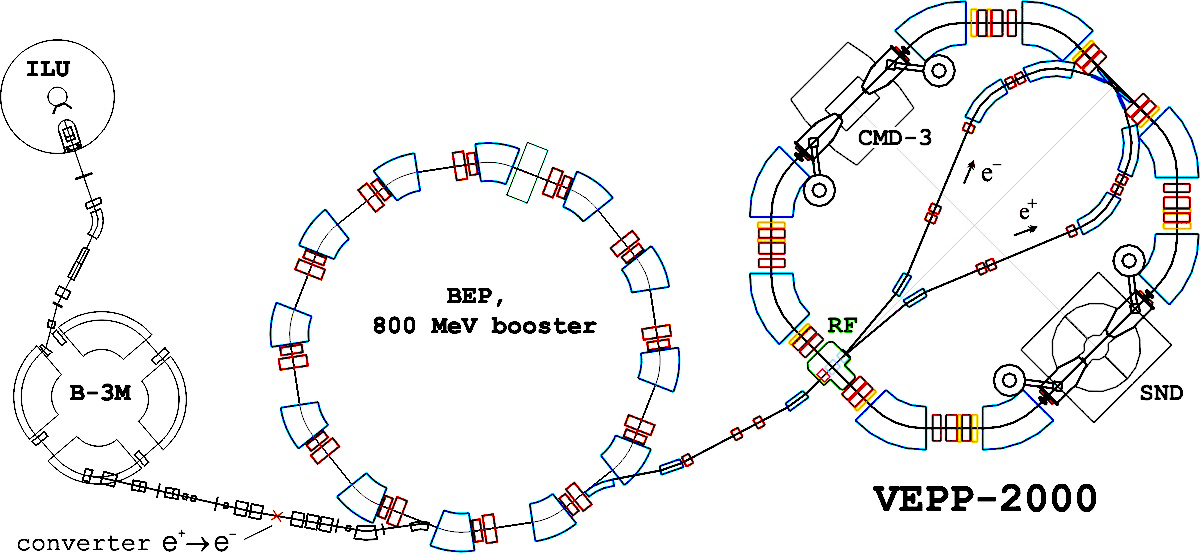
\includegraphics[width=\textwidth]{img/vepp2knew.png}
    \caption{Схема ускорительного комплекса ВЭПП-2000 до 2014 года.}
    \label{fig:vepp2000}
\end{figure}

Схема ускорительного комплекса до 2013 года представлена на Рис.~f\ref{fig:vepp2000}.
Комплекс состоял из импульсного линейного ускорителя ИЛУ,
синхротрон Б3-М,
конвертора,
бустурного кольца БЭП
и коллайдера ВЭПП-2000.

В 2013--2016 годах была проведена модернизация комлекса.
главным образом направленая на использования нового инжекционного комплекса ВЭПП-5
и улучшение БЭП,
позволяющие теперь ускорять и инжектировать пучки на энергии эксперимента,
то есть до \SI{1}{\GeVr}.

В 2017 году была возобновлена работа ускорительного комплекса и достигнуты значения светимости
\SI{3e31}{\cmr^{-2} \sr^{-1}} на энергии $\sqrt{s} = \SI{2}{\GeVr}$ \cite{Shatunov:2018xfm}.

В местах встречи пучков на коллайдере установлено и работает два универсальных детектора КМД-3 и СНД.



%\subsubsection{Измерение энергии пучков}

Для измерения энергии пучков на коллайдере ВЭПП-2000 используется метод с обратным комптоновским рассеянием монохроматичных фотонов \ce{CO}-лазера на электронном пучке, \cite{laserBeamAbakumova2014}.
Что позволяет измерять энергию пучков с относительной систематической ошибкой порядка \num{6e-5}.


% Для проверки корректности работы лазера и для определения энергии для статистики,
% набранной раньше установки и введения в работу лазера,
% используются измерения полной энергии системы с помощию процессов с присутствием заряженных частиц в конечном состоянии.

% Для определения энергии пучков по данным физических процессов используется измерение импульса заряженных частиц в дрейфовой камере.
% Заряженные каоны и пионы, а также протоны можно идентифицировать по удельному энерговыделению $dE/dx$ в дрейфовой камере и по выделившейся энергии в калориметре.
% Так как идентификация частиц основана разделении по $dE/dx$, то надо учитывать его зависимость от импульса частица.
% Также трек частицы в ДК должен иметь достаточно большую кривизну, для корректного определения импульса.
% В следствии этих причин, а также наличия порога реакций, лежащих в области сканирования ВЭПП-2000, для каждого процесса есть область применимости для определения энергии $e^+e^-$--пучков.
% Таким образом:
% \begin{itemize}
%   \item $e^+ e^- \to e^+ e^-$ используется в диапозоне $ \SI{}{\MeVr} < \sqrt{s} < \SI{}{\MeVr} $
%   \item $e^+ e^- \to K^+ K^-$ используется в диапозоне $ \SI{}{\MeVr} < \sqrt{s} < \SI{}{\MeVr} $
%   \item $e^+ e^- \to K^+ K^- \pi^+ \pi^-$ используется в диапозоне $ \SI{}{\MeVr} < \sqrt{s} < \SI{}{\MeVr} $
%   \item $e^+ e^- \to p \bar{p}$ используется в диапозоне $ \SI{}{\MeVr} < \sqrt{s} < \SI{}{\MeVr} $
% \end{itemize}

\newpage
\subsection{КМД-3}
\label{sec:cmd3}

\begin{figure}[htbp]
    \centering
    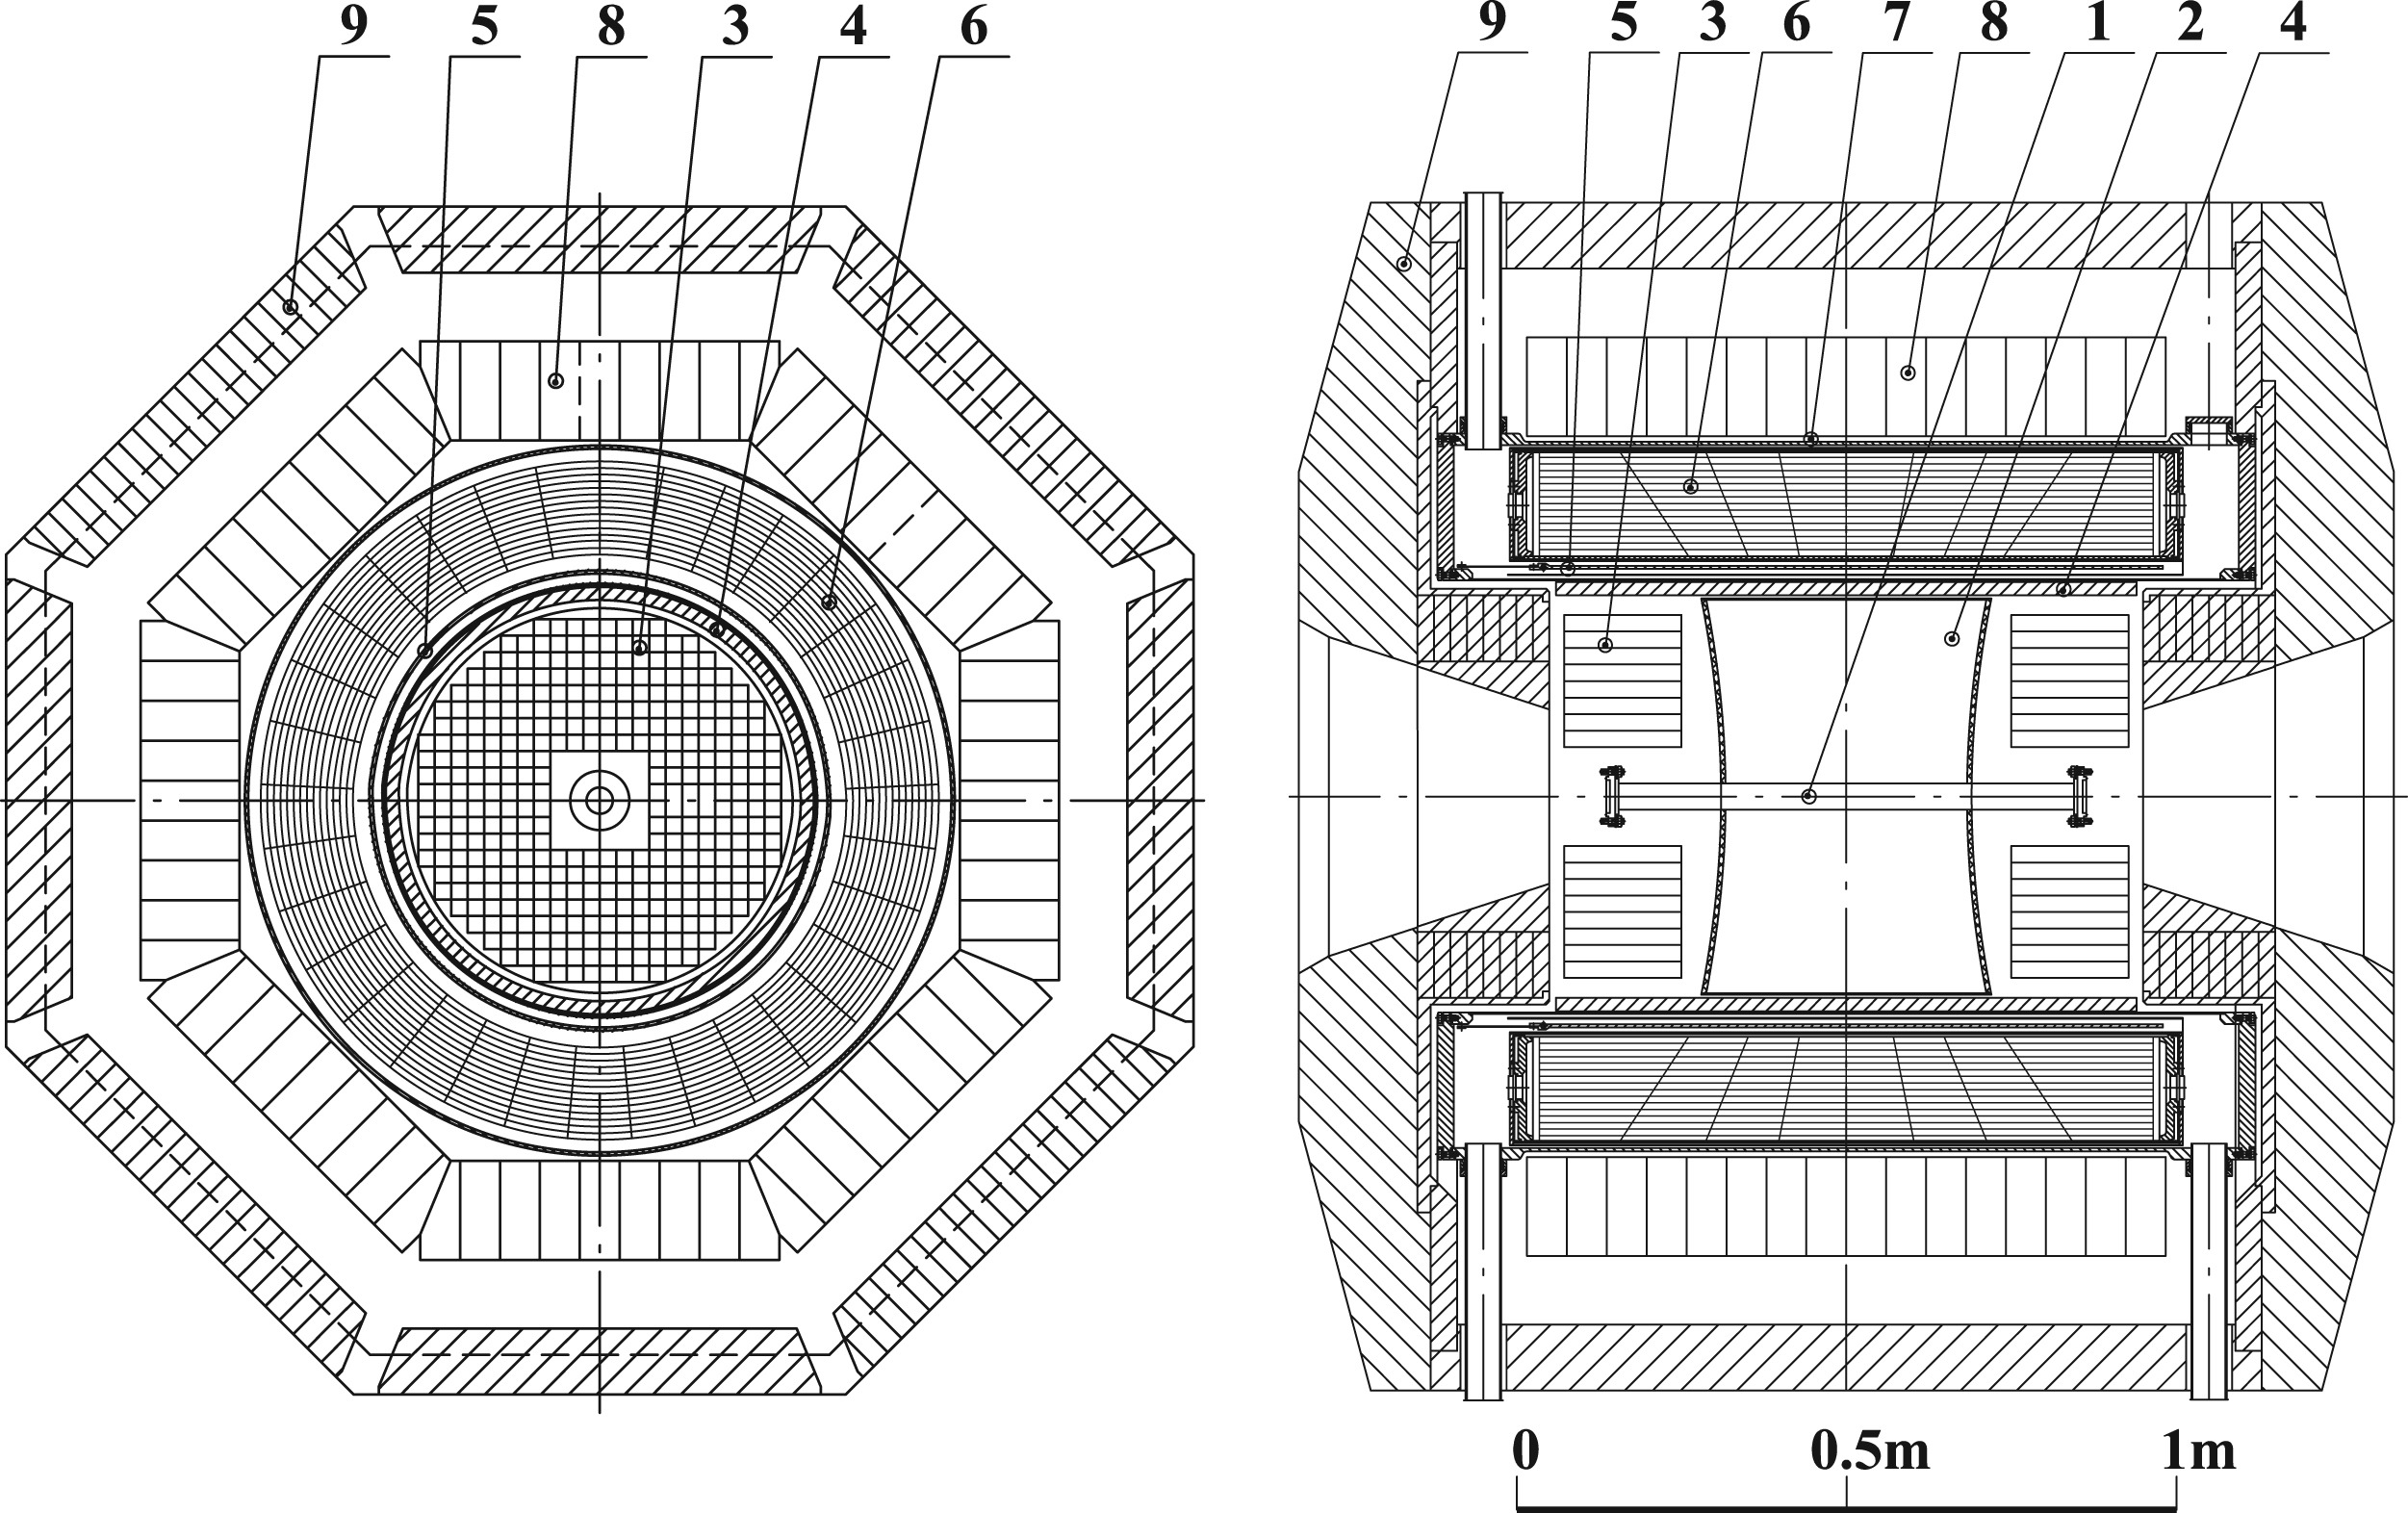
\includegraphics[width = .9\textwidth]{img/cmd3_detector/cmd3_layout.jpeg}
    \caption{Схема детектора КМД-3:
    	1 --- вакуумная труба,
    	2 --- дрейфовая камера,
    	3 --- \ce{BGO} калориметр,
    	4 --- Z-камера,
    	5 --- сверхпроводящий соленоид,
    	6 --- \ce{LXe} калориметр,
    	7 --- время-пролётная система,
    	8 --- \ce{CsI} калориметр,
    	9 --- ярмо магнита.
    }
    \label{fig:cmd3}
\end{figure}


Для проведения экспериментов на электрон-позитронном коллайдере \mbox{ВЭПП-2000} был частично модернизирован детектор СНД и создан новый универсальный детектор,
который получил название криогенного магнитного детектора третьего поколения
---
КМД-3 \cite{Khazin2010},
позволяющий регистрировать и измерять с высокой точностью параметры заряженных частиц и фотонов.
В период работы с 2011 года детектором КМД-3 было набаран интеграл светимости \SI{120}{\pbarnr^{-1}}.
Общий вид детектора представлен на Рис.~\ref{fig:cmd3}.
Электронные и позитронные пучки сталкиваются в центре вакуумной камеры (1), которая имеет внутренний диаметр \SI{34}{\mmr}. 
Центральная часть вакуумной камеры сделана из алюминия толщиной \SI{0.5}{\mmr} (\SI{5.3e-3}{\Xrad}\footnote{\si{\Xrad} --- радиационная единица длины.}) и длиной \SI{20}{\cmr}.

Для определения координат,
углов и импульсов заряженных частиц область столкновения пучков
охватывает трековая система,
которая находится внутри тонкого сверхпроводящего соленоида (толщина
\SI{0.18}{\Xrad},
магнитное поле \SI{1.3}{\teslaru}). 
Трековая система состоит из дрейфовой камеры,
Z-камеры и торцевого калориметра на основе кристаллов ортогерманата висмута \ce{Bi4Ge3O12}.
Вне магнитного поля в цилиндрической части детектора находятся жидко-ксеноновый калориметр \ce{LXe}(6)
и калориметр на основе активированных кристаллов \ce{CsI}(7). 
Жидко-ксеноновый калориметр позволяет измерить координаты точки конверсии фотона и совместно с калориметром на основе активированных кристаллов \ce{CsI} измерить энергию фотона.
Для фотонов, летящих из места встречи пучков, все три калориметра покрывают \SI{95}{\percent} телесного угла.
Между жидко-ксеноновом калориметром и \ce{CsI} калориметром расположена время-пролётная система (7).
Снаружи детектор окружен мюонной пробежной системой (8) на основе сцинтилляционных счётчиков для
подавления фона космических частиц.

%-----------------------------------
%	SUBSECTION Дрейфовая камера
%-----------------------------------

\subsubsection{Дрейфовая камера}
\label{sec:dc}

Дрейфовая камера (ДК) детектора КМД-3 способна работать при высоких загрузках и эффективно регистрировать многотрековые события, \cite{driftChCMD3Grancagnolo2010}. 
Координаты, углы и импульсы заряженных частиц измеряются в ДК,
которая плотно вставлена внутрь двухслойной многопроволочной пропорциональной Z-камеры (4). 
ДК представляет собой цилинидрический объём длиной \SI{44}{\cmr} и диаемтром \SI{60}{\cmr}.
Внутренняя и наружная цилиндрические оболочки,
а также торцевые фланцы сделаны из углепластика,
чтобы уменьшить количество пассивного вещества на пути частиц.
Торцевые фланцы выполенены в виде сегментов сферы.
Дрейфовая камера состоит из \num{1218} гексогональных ячеек с длиной диагонали \SI{18}{\mmr}.
Ячейка образована шестью полевыми проволочками с сигнальной проволочкой по центру.
Полевые проволочки имеют диаметр \SI{80}{\umr} и сделаны из титана, покрытого золотом. 
Сигнальные проволочки,
диаметром \SI{15}{\umr},
изготовлены из сплава вольфрам-кремний.
Камера продувается газовой смесью $\ce{Ar}:\ce{iC4H10}$ в пропорции $80:20$.
Суммарное количество вещества в ДК для частицы,
вылетевшей перпендикулярно по оношению к оси пучков,
эквиванлентно \SI{0.015}{\Xrad}.
Для частицы летящей вдоль оси $z$ из плоскости центрального сечения камеры
--- \SI{0.04}{\Xrad}.
Максимальное время дрейфа ионизации достигает \SI{600}{\nsr}.

Поперечные координаты трека измеряются по времени дрейфа первичной ионизации до сигнальных проволочек с точностью \SI{\sim 100}{\umr}.
Продольные координаты треков измеряются методом деления заряда и в среднем точность измерения составляет \SIrange{2}{3}{\mmr}. 

Поскольку камера расположена в магнитном поле,
в стандартном режиме работы \SI{1.3}{\teslaru},
то по кривизне треков заряженных частиц определяется их импульс и знак электрического заряда.

Абсолютная калибровка шкалы (пересчёт отношения зарядов на концах проволочки в продольную координату) осуществляется с использованием информации с Z-камеры,
которая имеет точность восстановления продольных координат трека \SI{\sim 0.5}{\mmr},
а систематическую погрешность меньше \SI{0.1}{\mmr}.
Импульсное разрешение ДК составило
$\sigma_p / p = \SIrange{1.3}{4.5}{\percent}$
для импульсов лежащих в диапазоне
\SIrange{160}{1000}{\MeVr \per \clight} (см. Рис.~\ref{fig:dc_mom_res}).
Разрешение по азимутальному углу равно \SI{9}{\mradianru} и \SI{3.5}{\mradianru}
для частиц с импульсами \SI{160}{\MeVr \per \clight} и \SI{1}{\GeVr \per \clight},
соответственно.
Разрешение по полярному углу практически не зависит от величины импульсы
и равно \SI{\sim 15}{\mradianru}.
Точность определения велечины удельных энергопотерь $\dif E / \dif x$
эквивалентна \SIrange{10}{13}{\percent}.
% Таким образом для частиц с импульсом \SI{500}{\MeVr \per \clight} разрешение составляет \SI{2.5}{\percent}


\begin{figure}
    \centering
    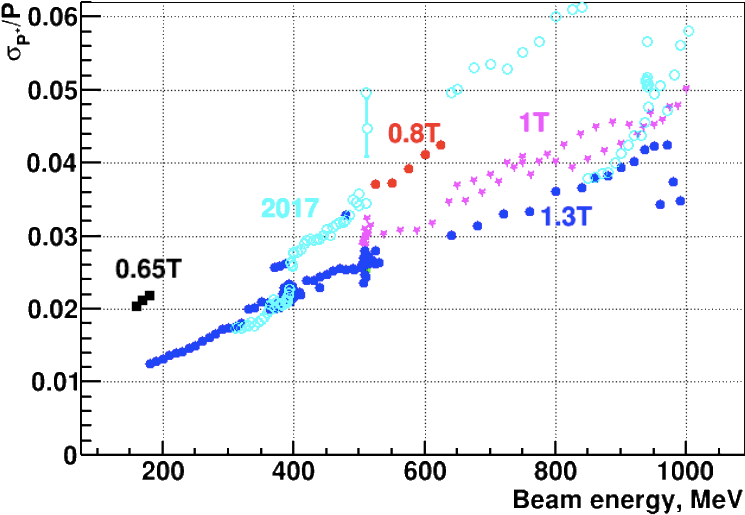
\includegraphics[height=.5\textwidth]{img/cmd3_detector/dc_mom_res.png}
    \caption{Импульсное разрешение дрейфовой камеры.}
    \label{fig:dc_mom_res}
\end{figure}


%-----------------------------------
%	SUBSECTION Z-камера
%-----------------------------------

\subsubsection{Z-камера}

Z-камера это двухслойная многопроволочная пропорциональная камера с анодным и катодным считыванием информации, \cite{Anashkin1992}.
Z-камера детектора КМД-3 является не только координатным детектором,
но и одним из основных элементов первичного заряженного триггера.
В каждом слое камеры \num{704} анодных проволочек, объединенных в $24$ сектора.
Камера продувается быстрой газовой смесью на основе фреона-14 \ce{CF4} и изобутана \ce{iC4H10} в пропорции $80:20$,
что позволяет достигнуть временной разброс анодных сигналов меньше \SI{5}{\nsr}.

Два слоя Z-камеры обеспечивают практически \SI{100}{\percent} эффективность регистрации заряженной частицы,
что особо важно для выроботки первичного сигнала заряженного триггера.
% Использование Z-камеры в первичном триггере предъявляет повышенные требования к ее эффективности.
% Наличие у камеры двух независимых слоёв позволяет обеспечить практически \SI{100}{\percent} эффективность запуска.
% Поскольку Z-камера расположена внутри цилиндрического калориметра, необходимо, чтобы она содержала минимальное количество вещества.
% Характерный масштаб задается толщиной сверхпроводящего магнита, составляющего основную массу вещества перед калориметром (примерно \SI{0.18}{\Xrad}).
Так как Z-камера находится перед цилиндрическим калориметро,
то во избежание ухудшения энергетического разрешения калориметра,
конструкция Z-камеры оптемизировалась по количеству используемого вещества и составила в среднем \SI{0.02}{\Xrad} для нормально падающей частицы,
что заметно меньше толщины сверхпроводящего соленоида (\SI{0.18}{\Xrad}),
находящегося также перед цилиндрическим калориметром.

%-----------------------------------
%	SUBSECTION Цилиндрический калориметр
%-----------------------------------

\subsubsection{Цилиндрический калориметр}
\label{sel:barrel_calorimeter}

Цилиндрический калориметр детектора КМД-3 состоит из двух слоёв и перекрывает полярные углы от \ang{38} до \ang{142},
охватывая \SI{79}{\percent} полного телесного угла,
\cite{BarrelCalCMD3Anisenkov:2013yva}.
Общая толщина активного вещества для нормально падающей частицы составляет \SI{13.3}{\Xrad}.
Внутренний слой представлен жидко-ксеноновым калориметром,
а внешний
---
кристаллическим калориметром на основе \ce{CsI(Na)} и \ce{CsI(Tl)}.

Толщина ближнего к оси пучков жидко-ксенонового калориметра составляет \SI{5.2}{\Xrad},
масса ксенона \num{1.2} тонны. 
Второй,
внешний калориметр построен на основе кристаллов \ce{CsI(Na)} и \ce{CsI(Tl)} общим числом \num{1152} и весом равен \num{2.2} тонны, 
радиационная длина \SI{8.1}{\Xrad}.

Суммарно перед активном веществом калориметра находится 
\SI{6.27}{\gr \per \cubed \cmr} или \SI{0.35}{\Xrad} пассивного вещества.
Между кристаллическим и жидким калориметром находится 
\SI{4.63}{\gr \per \cubed \cmr} или \SI{0.25}{\Xrad}.

Энергетическое разрешение цилиндрического калориметра для событий баба рассеяния описывается функцией
$\sigma_E^{\text{bar}} / E = \frac{ \SI{3.6}{\percent} }{ \sqrt{ E / \si{\GeVr} } } \oplus \SI{2.7}{\percent}$
(см. Рис.~\ref{fig:cal_energy_resolution}), \cite{Anisenkov:2017pgv}.
Пространственное разрешение цилиндрического калориметра для кластеров с восстановленной точкой конверсией по полоскам \ce{LXe} калориметра описывается функцией
$\sigma_{\varphi} / \si{\mradianru} = 3.70 + 0.33 / (0.25 + E / \si{\GeVr})$ (см. Рис.~\ref{fig:cal_spatial_resolution}).
В отсутствие полосковой информации
---
$\sigma_{\varphi} / \si{\mradianru} = 37.0 + 3.6 / (0.1 + E / \si{\GeVr})$.

% В соответствии с моделированием для $\gamma$-квантов с энергией \SI{350}{\MeVr} доля энергии,
% выделившейся в \ce{CsI} калориметре,
% составляет \SI{\sim 20}{\percent},
% для фотона с энергией \SI{950}{\MeVr}
% ---
% уже около \SI{30}{\percent}.

%-----------------------------------
%	SUBSUBSECTION Жидко-ксеноновый калориметр
%-----------------------------------

\paragraph{Жидко-ксеноновый калориметр}
\label{sec:lxe}

\begin{figure}[htbp]
    \begin{minipage}[t]{0.27\textwidth}
        \centering
        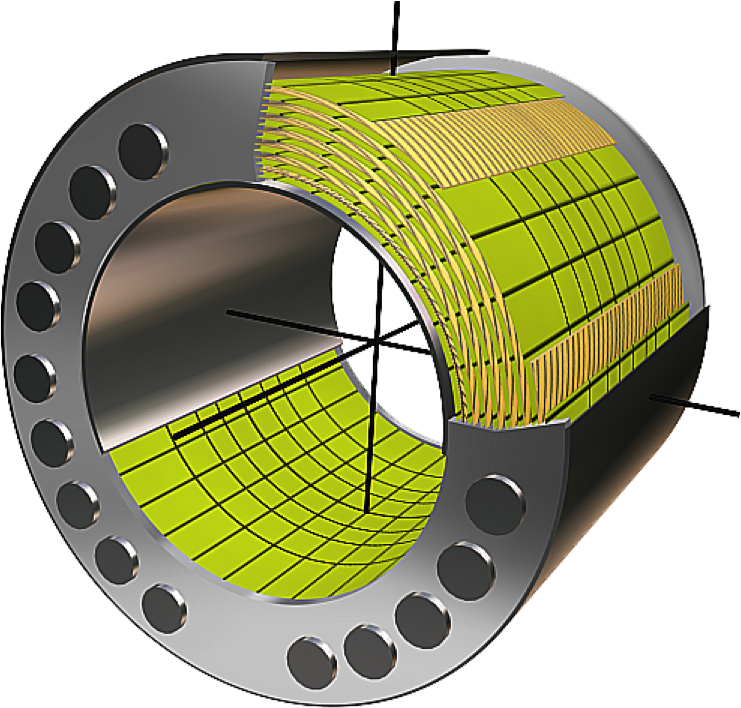
\includegraphics[width=\textwidth]{img/cmd3_detector/lxe_sketch.png}
        \label{fig:lxe_sketch}
        \caption{Жидкоксеноновый калориметр.}
    \end{minipage}
    \hfill
    \begin{minipage}[t]{0.68\textwidth}
        \centering
        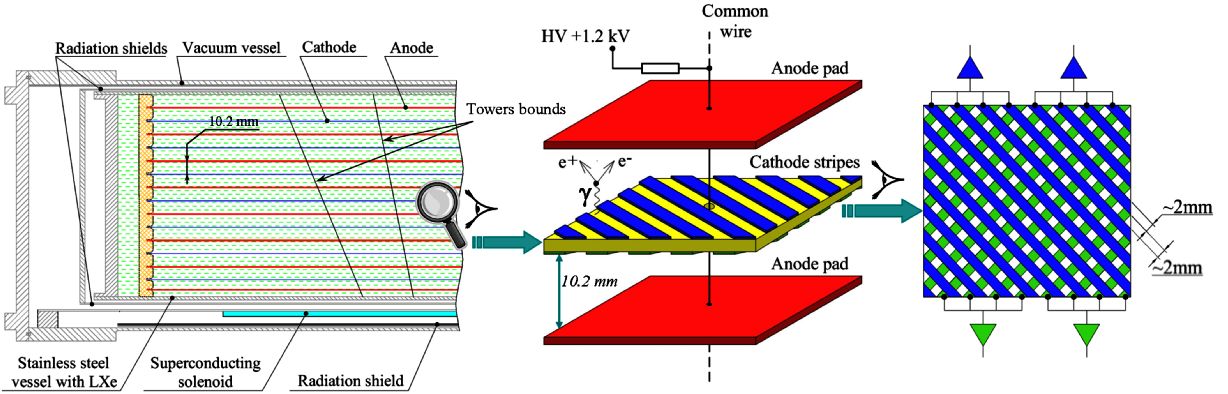
\includegraphics[width=\textwidth]{img/cmd3_detector/lxe_electrode_structure.png}
        \label{lxe_electrode_structure}
        \caption{Электроника жидкоксеновового калориметра.}
  \end{minipage}
\end{figure}

Жидко-ксеноновый калориметр показан на Рис.~\ref{fig:lxe_sketch},
и состоит из 15 соосных цилиндров,
семь из которых имеют полосковую структуру и являются катодами,
а восемь цилиндров образуют аноды.
Медная фольга каждого анода разделена на 8 колец вдоль оси пучка.
Каждое кольцо, в свою очередь,
поделено на \num{33} одинаковых сегмента в $R-\varphi$ плоскости. 
Образованные таким образом прямоугольники,
электрически соединены по радиусу и образуют башни в количестве \num{264}, каждая из которых смотрит на точку взаимодействия пучков.
Зазор между анодом и катодом \SI{10.2}{\mmr}.
% и при рабочем напряжении $\sim 1500$~В время дрейфа электронов составляет $\sim 4.5$~мкс.
Диаметры внутреннего и наружного цилиндров равны \SI{738}{\mmr} и \SI{1024}{\mmr} соответственно,
длина \SI{920}{\mmr}. 

Каждый катодный электрод на обоих сторонах разделен на полоски,
которые по отношению к оси пучков составляют углы \ang{\pm 45}. 
Каждая полоска, в свою очередь,
подразделена на 4 узких полоски шириной \SI{2}{\mmr} и зазором между ними \SI{2}{\mmr}. 
Такая структура полосок полупрозрачна и индуцированный сигнал практически одинаков на обеих сторонах катода. 
В результате обе координаты точки конверсии фотона могут быть измерены в одном зазоре.
Полное число катодных каналов \num{2124}.

Координатное разрешение измерялось по отобранным коллинеарным событиям,
используя аналоговую информацию с полосок. 
Координаты трека в каждом зазоре определяются методом центра тяжести,
через которые проводится оптимальная прямая
линия. 
В результате было показано,
что пространственное разрешение составляет \SIrange{\sim 1}{2}{\mmr}.


%-----------------------------------
%	SUBSUBSECTION Калориметр на основе кристаллов CsI
%-----------------------------------

\paragraph{Калориметр на основе кристаллов CsI}
\label{sec:csi}

\begin{figure}[htbp]
    \begin{minipage}[t]{0.35\textwidth}
        \centering
        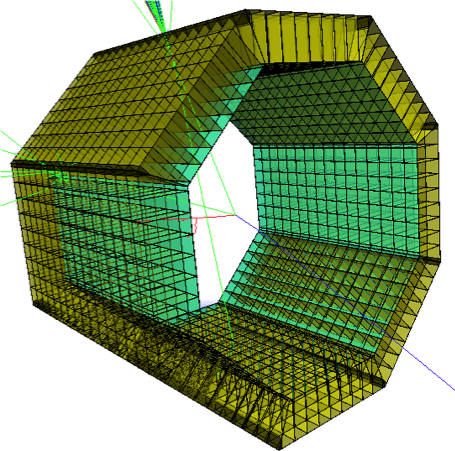
\includegraphics[width=\textwidth]{img/cmd3_detector/csi_scketch.png}
        \label{fig:lxe_sketch}
        \caption{\ce{CsI} калориметр.}
    \end{minipage}
    \qquad
    \begin{minipage}[t]{0.60\textwidth}
        \centering
        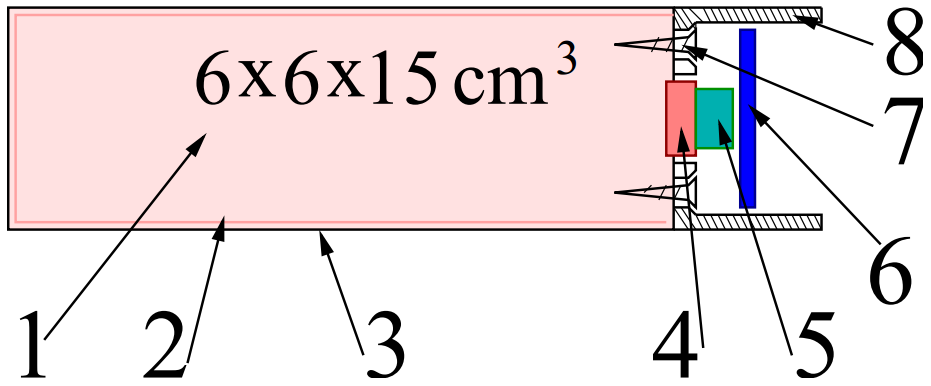
\includegraphics[width=.9\textwidth]{img/cmd3_detector/csi_crystal_scheme_v2.png}
        \label{lxe_electrode_structure}
        \caption{Счётчик \ce{CsI} калориметра:
        1 --- сцинтилляционный кристалл,
        2 --- белый пористый тефлон Gore-Tex,
        3 --- алюминизированный лавсан,
        4 --- pin-фотодиод,
        5 --- резиновый уплотнитель,
        6 --- предусилитель,
        7 --- шуруп,
        8 --- стальная рама.}
  \end{minipage}
\end{figure}


Калориметр на основе кристаллов \ce{CsI(Tl)} и \ce{CsI(Na)} состоит из 8 одинаковых октантов и каждый содержит 9 линейных модулей с \num{16} кристаллами, ориентированных вдоль оси пучков,
\cite{Aulchenko:2015msa}.
Зазор между кристаллами составляет не более \SI{0.5}{\mmr}.
Семь центральных модулей состоят из прямоугольных кристаллов с размерами $60 \times 60 \times \SI{150}{ \cubic\mmr}$.
Два боковых модуля имеют специальную форму кристаллов, чтобы обеспечить плотное сочленение двух соседних октантов без зазоров. 
Регистрация светового сигнала с каждого сцинтилляционного кристалла производится с помощью полупроводникового PIN фотодиода S2744-8 фирмы Hamamatsu Photonics с чувствительной площадью $1 \times \SI{2}{\square\cmr}$. 
Токовые сигналы с фотодиодов поступают на входы зарядочувствительных предусилителей,
размещённых непосредственно около фотодиодов и дающих на выходе парафазный сигнал.
По витой паре сигнал поступает на плату усилителей-формировщиков-оцифровщиков УФО-32,
способную обслуживать до двух линеек.
В плате после аттенюатора сигнал делится на две части.
Первая служит для выработки триггерного сигнала,
для чего в плате формируется \num{5} сигналов суммарного энерговыделения,
которые поступают на плату амплитудных дискриминаторов и сумматоров АДИС,
формирующих сигнал о срабатывание калориметра для последующего использования в триггере детектора.



\begin{figure}[htbp]
    \begin{minipage}[t]{0.475\textwidth}
        \centering
        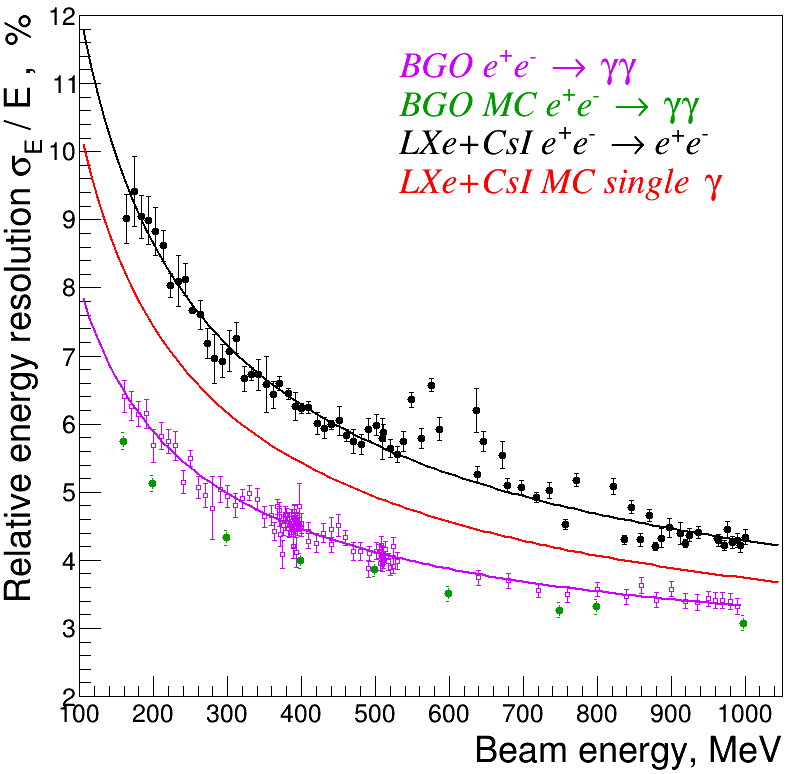
\includegraphics[width=\textwidth]{img/cmd3_detector/comb_energy_resolution.png}
        \label{fig:cal_energy_resolution}
        \caption{Энергетическое разрешение калориметров.}
    \end{minipage}
    \hfill
    \begin{minipage}[t]{0.475\textwidth}
        \centering
        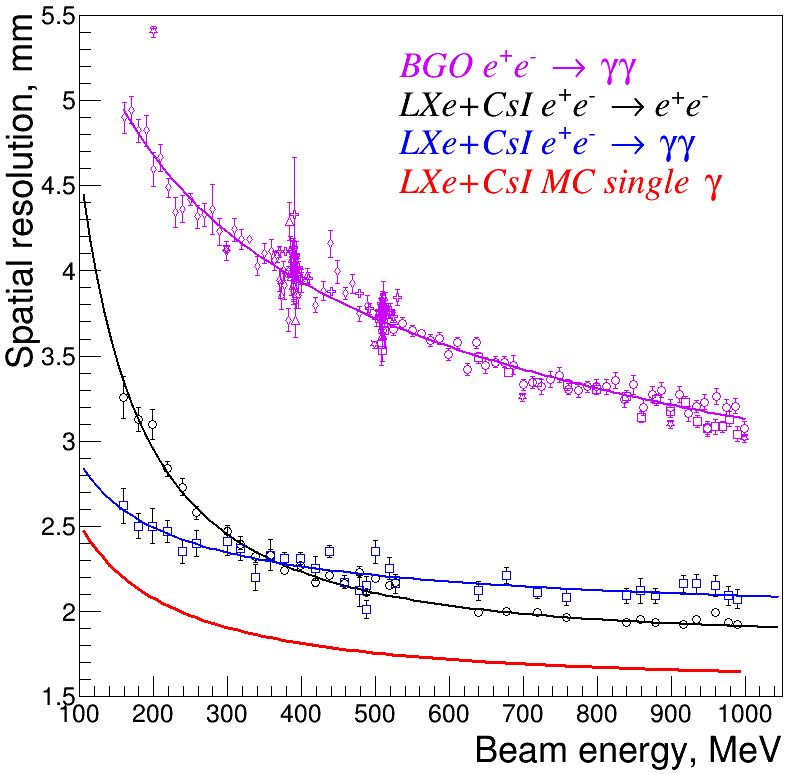
\includegraphics[width=\textwidth]{img/cmd3_detector/comb_spatial_resolution.png}
        \label{fig:cal_spatial_resolution}
        \caption{Пространственное разрешение калориметров.}
  \end{minipage}
\end{figure}



%-----------------------------------
%	SUBSECTION Торцевой калориметр на основе кристаллов BGO
%-----------------------------------

\subsubsection{Торцевой калориметр на основе кристаллов BGO}
\label{sec:bgo}

\begin{figure}[htbp]
    \begin{minipage}[t]{0.475\textwidth}
        \centering
        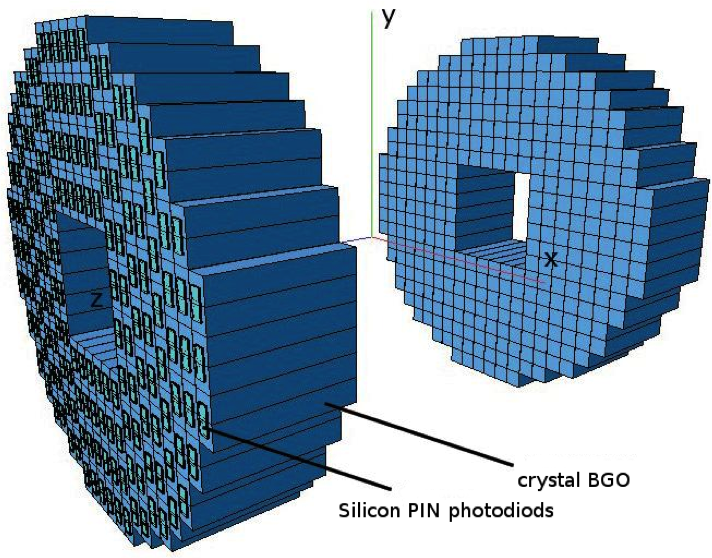
\includegraphics[width=\textwidth]{img/cmd3_detector/bgo_scetch.png}
        \label{fig:cal_energy_resolution}
        \caption{\ce{BGO} калориметр.}
    \end{minipage}
    \hfill
    \begin{minipage}[t]{0.475\textwidth}
        \centering
        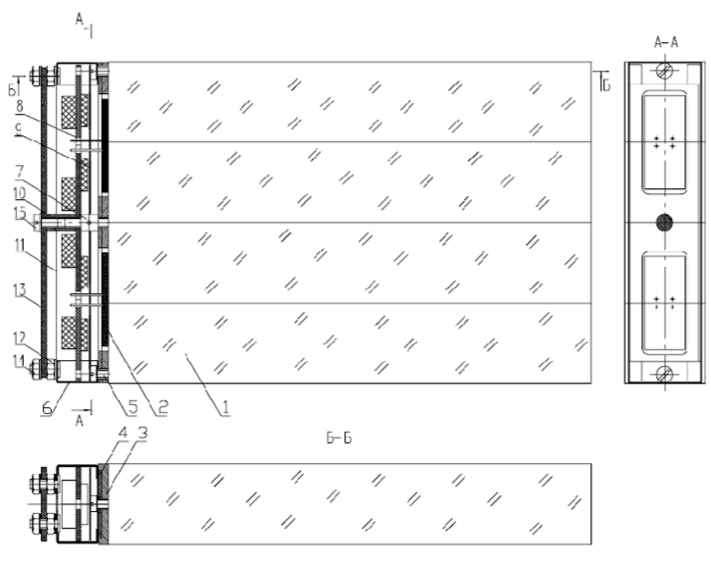
\includegraphics[width=\textwidth]{img/cmd3_detector/bgo_module_scheme.png}
        \label{fig:cal_spatial_resolution}
        \caption{Схема модуля \ce{BGO} калориметра.}
  \end{minipage}
\end{figure}

Торцевой калориметр на основе кристаллов ортогерманата висмута \ce{Bi4Ge3O12} (\ce{BGO}) представляет из себя два диска, расположенных вплотную к торцам ДК, \cite{BGOAkhmetshin2009}.
По центру этих дисков имеются отверстия для вакуумной камеры и компенсирующих магнитов.
Калориметр перекрывает полярные углы,
отсчитанные от оси пучков,
от \ang{16} до \ang{49} и от \ang{131} до \ang{164} и покрывает примерно \SI{30}{\percent} от полного телесного угла.
Для фотонов с энергиями 
\SIrange[range-phrase = --, range-units = single]{100}{700}{\MeVr}
энергетическое разрешение составляет 
\SIrange[range-phrase = --, range-units = single]{\sim 4}{8}{\percent},
а угловое разрешение \SI{\sim 0.02}{\radianru}.
Каждый диск состоит из \num{340} одинаковых кристаллов с размерами
\SI[product-units = power]{25 x 25 x 150}{\mmr}
и общим весом
\SI[product-units = single]{2 x 225}{\kgr}. 
Радиационная толщина калориметра для нормально падающих частиц составляет \SI{13.4}{\Xrad}.
Световой сигнал с каждого кристалла регистрируется полупроводниковым фотоприемниками S3590-08 фирмы Hamamatsu Photonics
с чувствительной областью \SI[product-units = power]{1 x 1}{\cmr},
имеющие высокую квантовую эффективность и стабильность в работе. 
Измерения показали,
что световыход составляет \SI{\sim 600}{\elementarycharge\per\MeVr},
а электронный шум \SI{\sim 500}{\elementarycharge},
что эквивалентно \SI{\sim 0.8}{\MeVr}.
Температура калориметра стабилизируется с помощью водного охлаждения.



%-----------------------------------
%	SUBSECTION Мюонная пробежная система
%-----------------------------------

\subsubsection{Мюонная пробежная система}
\label{sec:mu}

Мюонная пробежная система состоит из \num{36} сцинтилляционных счетчика и расположена с наружи магнитного ярма.
Мюоны с энергией больше \SI{550}{\MeVr},
рожденные в $e^+e^-$-столкновениях,
будут долетать до этих счетчиков. 
Каждый счетчик имеет размеры \SI[product-units = power]{2 x 20 x 150}{\cmr} и просматривается с каждой стороны двумя ФЭУ-84.
Сигналы с ФЭУ усиливаются и оцифровываются в платах TQ. 
На этой системе получено временное разрешение \SI{\sim 1}{\nsr}, что достаточно для подавления космических событий, имеющих время пролета через детектор \SI{\sim 7}{\nsr}.


%-----------------------------------
%	SUBSECTION Время-пролетные счетчики
%-----------------------------------

\subsubsection{Время-пролетные счетчики}
\label{sec:tof}

Время-пролетные счетчики [???], на основе сцинтиллятора ВС-406 фирмы <<БАЙКРОН>> расположены в
узком зазоре (\SI{7}{\mmr}) между ксеноновым и \ce{CsI} калориметрами и предназначены для регистрации продуктов
аннигиляции антинейтронов, рождающихся в реакции $e^+e^- \to n \bar{n}$. 
Всего \num{16} одинаковых счетчиков с размерами \SI[product-units = power]{0.5 x 20 x 90}{\cmr},
каждые два из которых крепятся на лицевой стороне \ce{CsI} калориметра,
образуя замкнутый октант.
Каждый счетчик просматривается двумя компактными фотоприемниками,
сделанных на основе микроканальных пластин
(МКП, диаметр --- \SI{30}{\mmr}, высота --- \SI{17}{\mmr}). 
Прямо на корпусе МКП смонтирован высоковольтный делитель и предусилитель с полосой пропускания \SI{\sim 1}{\GHzr}. 
Сигналы с МКП поступают на входы плат TQ (\num{16} каналов),
где они усиливаются и оцифровываются. 
На этой системе получено временное разрешение \SI{\sim 1}{\nsr}.




\subsubsection{Система запуска детектора}
\label{sec:trigger}

Система запуска детектора делится на две части,
одна из которых --- процессор поиска треков (ППТ) --- направлена на регистрацию событий с заряженными частицами,
в то время как другая --- процессор поиска энергетических кластеров (ППЭК) --- ориентирована на срабатывания от нейтральных частиц.
Первый процессор получает информацию от интерфейсов первичного триггера ЗК и ДК.
Второй от амплитудных дискриминаторов и сумматоров каждого из калориметров.
Инфомация с процессорв посика поступает на триггерную плату,
которая вырабатывает сигнал общего стопа для системы сбора данных,
по которому происходит вычитывание всех каналов электроники детекора.

ППЭК анализирует энергетическое распределение с различными шаблонами срабатывания --- масками ---
и в случае одного или более совпадений вырабатывает сигнал нейтрального триггера.
Всего используется 7 масок.
Три из них направлены на отбор коллинеарных событий в торцевом калориметре.
Остальные маски обрабатывают информацию с цилиндрического калориметра:
\begin{itemize}
    \item 2 кластера в разных половинах по $z$ с суммарным энерговыделением более \SI{200}{\MeVr};
    \item не менее 3 кластеров в разных половинах по $z$ с суммарным энерговыделением более \SI{100}{\MeVr};
    \item срабатывания и в \ce{LXe}, и \ce{CsI} калориметре с энерговыделением более \SI{200}{\MeVr};
    \item NTN
\end{itemize}







\subsubsection{Система сбора данных}
\label{sec:daq}

При срабатование триггера детектора происходит вырабатывание сигнала общего стопа,
по кторому происходит вычитывание всех каналов электроники.
Информация по C-Link'ам поступает в блоки приёма-передачи данных (БППД).
Последние организованны в древовидную структуру с передачей данных по Ethernet.
Информация с последнего БППД передаётся на персональный компьютер,
где в сырых данных происходит подавление нулей,
уменьшающая их первоначальный размер в $\sim 10$ раз.
Затем происходит формировка события,
когда информация с различных систем группируется из всего потока данных в одно место и записывается в файл.
Типичный размер события составляет 10\,кБ.
События записываются в файлы по 2\,ГБ (\num{\sim 200000} событий).
После чего происходит копирование файлов в распределённое хранилище данных с созданием одной резервной копии в нём.
Регулярно просиходит создрания резервных копий на лентах долгого хранения.

Вместе с набором основных данных идёт мониторирования основных параметров детектора и качества набора данных,
позволяющее оперативно выявлять и устронять неполадки.




\subsubsection{Программа реконструкции событий}
\label{sec:event_reco}


Для проведения анализа физических процессов информация,
записанная во время эксперимента,
должна быть преобразована в физические характеристики события
(число частиц,
их энергии и импульсы с направления,
параметры,
характеризующие тип частицы и т.\,п.).


\paragraph{Реконструкция событий в координатной системе}

Реконструкция событий в трековой системе состоит из восстановления треков заряженных частиц и поиска их общих вершин.
Данная процедура подробно описана в работах \cite{Karawdina:2007:track_reco}.


Первым шагом проводится процедура гистограммирование сработавших проволочек
в плоскости $\rho$--$\phi$ по параметрам $\rho$ и $\varphi$ относительно начала координат
--- положения пучка.

Первым шагом проводится процедура гистограммирование сработавших проволочек,
отдельно в плоскости $\rho$--$\phi$ и отдельно в плоскости $z$--$\rho$.
Для чего отбираются 3--4 рядом сработавшие ячейки.
Выбирается наиболее вероятное направлние трека и произвольным образом координаты одной из сработавших ячеек беруться за начала координат для процедуры гистограммирования,
в ходе которой строится распределения по углу хитов.
Напраление трека,
к которому принадлежит первичный кластер сработавших проволочек,
определяет пик в распределении и хиты,
отвечающую наивероятнейшему углу,
присовокупляются к кластеру.
Полученая группа хитов является кандидатом на трек.

Кандидаты с количеством хитов не менее пяти аппроксимируются соответственно окружностью и прямой
путём минимизации нормализованных квадратов отклонений измеренных параметров от предсказания функций.
После этого идёт поиск до сих пор не принадлежащих ни к одному треку сробатаваний проволочек в ДК.
Надйденые хиты присоединяются к ближайшему концевому хиту трека при условии,
что расстояния между координатой найденной ячейки и хитом трека меньше \SI{3}{\cmr},
а отколение по времени дрейфа и $z$-координате меньше $5 \sigma_t$
и $5 \sigma_z$, соответственно.




\paragraph{Реконструкция кластеров в электромагнитном калориметре}


В ходе эксперимента с калориметров записываются все сигналы с каждого кристалла \ce{BGO} или \ce{CsI} калориметров,
и с башен и полосок \ce{LXe} калориметра при превышении соответствующих порогов.
В ходе последующей реконструкции события восстановление кластеров энерговыделения можно разделить на несколько последовательных этапов.
\begin{enumerate}
    \item \label{itm:cluster_reco_1} Нахождение и образование кластеров в торцевом и \ce{LXe} калориметрах.
    Для чего в ходе калибровок определяется так называемые нижние $E_{\text{low}}$ и верхние пороги $E_{\text{high}}$.
    Далее ищется элемент с амплитудой сигнала превосходящий верхний порог $E_{\text{high}}$
    --- такой элемент называется затравочным.
    К затравочному элементу присоединяются все соседние элементы с сигналом превышающим нижний порог.
    Соседними называются кристаллы или башни имеющие смежную грань.
    Соседними полосками называются соседние полоски с одинаковой ориентацией находящиеся в одном слое.
    Когда закончено формирование кластера,
    происходит поиск следующего.
    Так повторяется пока не будут исчерпаны все элементы превышающие верхний порог и не входящие в уже найденные кластеры.
    \item Для каждого найденного кластера находится центр его тяжести.
    \item Поиск пересечений полосок в каждом слое по результатам которого формируется коллекция позиций возможных пересечений полосковых кластеров.
    \item Объединение башенных и полосковых кластеров в \ce{LXe} калориметре.
    К башенным кластерам прикрепляется информация с полосок,
    чьи пересечения лежат в пространстве башенного кластера.
    Те же пересечения,
    что не принадлежат ни одному из башенных кластеров считаются ложными и в дальнейшем не рассматриваются.
    \item В рамках гипотезы электромагнитного ливня порождённого фотоном находится точка конверсии фотона как точка пересечения полосковых кластеров,
    принадлежащая к данном жидкоксеноновому кластеру и ближайшая к оси $z$ детектора.
    При множественности таких пересечений выбирается то,
    что ближе всего к центру тяжести башенного кластера.
    \item Объединение кластеров \ce{CsI} и \ce{LXe} калориметров.
    Для всех башен каждого \ce{LXe} кластера ищутся соседние \ce{CsI} кристаллы
    с энерговыделением больше $E_{\text{low}}^{\ce{CsI}}$.
    Кристалл считается соседним если
    $ | \theta_{\ce{CsI}} - \theta_{\ce{LXe}} | < \delta_\theta^{\ce{CsI}} $
    и
    $ | \varphi_{\ce{CsI}} - \varphi_{\ce{LXe}} | < \delta_\varphi^{\ce{CsI}} $,
    где $\delta_\theta^{\ce{CsI}} = \delta_\varphi^{\ce{CsI}} = \SI{0.2}{\mradianru}$.
    Если кристалл соседний более,
    чем с одним ксеноновым кластером,
    то он присваивается \ce{LXe} с наибольшим энерговыделением.
    Соседние счётчики найденных таким образом кристаллов также присоединяются к ксеноновому кластеру.
    \item Все оставшиеся без-причастными от предыдущего шага кристаллы \ce{CsI} калориметра проходят процедуру по поиску и формировки кластеров описанных в пункте~\ref{itm:cluster_reco_1}.
    \item Если к \ce{LXe} принадлежит крайняя башня,
    то происходит присоединение к нему соседних кристаллов \ce{BGO} 
    с энерговыделением больше чем $E_{\text{low}}^{\ce{BGO}}$.
    Соседним кристалл считается если
    $ | \pi/2 - \theta_{\ce{BGO}} | < | \pi/2 - (\theta_{\ce{LXe}} + \delta_{\theta}^{\ce{BGO}}) | $
    и
    $ | \varphi_{\ce{BGO}} - \varphi_{\ce{LXe}} | < \delta_\varphi^{\ce{BGO}} $,
    где $\delta_\theta^{\ce{BGO}} = \SI{0.05}{\mradianru}$,
    а $\delta_\varphi^{\ce{BGO}} = \SI{0.1}{\mradianru}$.
    Если отобранный \ce{BGO} кристалл принадлежит к \ce{BGO} кластеру,
    то этот кластер следует за кристаллом и присоединяется к \ce{LXe} кластеру.
    \item Объединённому кластеру присваивается суммарная энергия всех входящих в него элементов.
    \item Координаты объединённого кластера определяются как координаты \ce{LXe} кластера,
    если в последним они восстановлены по полоскам и энерговыделение в \ce{LXe} превышает
    энерговыделение в \ce{BGO}.
    В остальных случаях координата ищется методом центра тяжести по всем элементам объединённого кластера.
    \item К кластерам применяются поправки,
    учитывающие утечки ливня и потери энергии в пассивном веществе.
    Также поправляются координаты кластера,
    что особенно существенно,
    когда оные были определены не по катодным палоскам \ce{LXe} калориметра.
\end{enumerate}




% %-----------------------------------
% %	SUBSECTION Система сбора данных
% %-----------------------------------

% \subsubsection{Система сбора, обработки и хранения данных}

% Аппаратная часть системы сбора данных (ССД) КМД-3 реализована с использованием специально разработанных для этой цели унифицированных функциональных узлов, \cite{SSD.Ruban.2009}.
% Основными компонентами электроники ССД являются Блоки первичной Обработки Сигналов (БОС),
% блоки приема/передачи данных (БППД) и электроника первичного триггера.
% Общая организация аппаратной части ССД представлена на рис. \textbf{схема}. 
% Все физические величины сигналов (заряды, амплитуды, времена) преобразуются в напряжения, которые оцифровываются с помощью АЦП. 
% % Преобразование сигналов от различных чувствительных устройств детектора в напряжения и их оцифровка осуществляется с помощью блоков обработки сигналов.
% БОС преобразуют сигналы от различных чувствительных устройств детектора и оцифровывают их.
% Всего в ССД используются 3 разновидности БОС: 
% \begin{itemize}
%   \item оцифровывающие времена прихода и амплитуды (заряды) сигналов;
%   \item оцифровывающие амплитуды калориметрических сигналов;
%   \item оцифровывающие зарядовые сигналы координатных полосок.
% \end{itemize}
% Все БОС, используемые в ССД многоканальные (до 48 каналов), оцифровка нескольких напряжений в них производится одним АЦП среднего быстродействия
% (\SI{\sim e6}{\textup{сигналов}/\sr}),
% который подключается к каждому каналу с помощью мультиплексора.
% % Все АЦП имеют быстродействие порядка \SI{e6}{сигналов/с}. 

% %Получаемые на выходе АЦП данные передаются в специально разработанную последовательную линию связи --- линк.
% Получаемые на выходе АЦП данные передаются по специально разработанной последовательной линии связии --- линк --- в БППД.
% % Эта же линия используется для управления блоками БОС и тестирования электроники ССД.
% Линк также используется для управления блоками БОС и тестирования электроники ССД.
% % Последовательные линки, выходящие с БОС, собираются на блоках приема/передачи данных (БППД).
% Основная функция БППД --- обеспечить управление и синхронизацию БОС, прием данных и их дальнейшую передачу в компьютеры ССД.
% % Для этой цели блоки БППД управляют работой БОС посредством командных посылок, передаваемых по последовательным линкам от БППД к БОС. 
% % Командная посылка состоит из кода операции и вспомогательных данных.
% % Так командная посылка Start\_Regular содержит номер события и инициирует запуск измерений в БОС с последующей передачей данных в БППД.
% Блоки БППД производят буферизацию и группируют полученные данные в пакеты для пересылки в компьютер (Frontend PC) через сеть Fast Ethernet.
% % Кадр протокола взаимодействия с БППД непосредственно вкладывается в поле данных кадра Ethernet.
% % При этом полезная информация, передаваемая в компьютер, состоит из последовательности оцифрованных значений, полученных от соответствующих БОС.

% Первичный триггер (ПТ) КМД-3 работает по схеме с <<общим стопом>>, \cite{Trigger.Ruban.2007}.
% Это означает, что платы БОС самостоятельно отслеживают появление сигналов от чувствительных элементов детектора и запоминают их до поступления сигнала триггера. 
% % В качестве оценки времени принятия решения ПТ используется промежуток от момента появления сигналов анодных проволочек Z-камеры до момента выработки сигнала триггера (в силу высокой плотности проволочек и, следовательно, маленького времени дрейфа).
% Электроника ПТ состоит из 2 слабо связанных частей: <<заряженного>> триггера, обрабатывающего сигналы от трековой системы детектора, и <<нейтрального>> триггера, обрабатывающего сигналы от калориметров.
% % Работа ПТ синхронизована с сигналом <<фазы>> пучков в накопителе ВЭПП-2000.
% % Таким образом, обеспечивается временная привязка команды запуска оцифровки к моменту столкновения пучков в накопителе, при котором произошло выбранное событие.
% Работа ПТ синхронизирована с сигналом <<фазы>> пучков в накопителе ВЭПП-2000, тем самым обеспечивая временную привязку команды запуска оцифровка к столкновению пучков.
% % Команда о запуске измерений раздается триггером через блоки приема/передачи данных в блоки БОС.
% % Для синхронизации данных применяется аппаратная нумерация событий внутри захода.
% % Счётчик номера события находится в триггере и раздается вместе с командой о запуске. 
% % Каждый блок БОС приписывает номер события к порции данных, относящихся к текущему событию.
% % Итак, тракт данных аппаратной части ССД состоит из плат БОС, оцифровывающих сигналы от чувствительных систем детектора, блоков БППД, коммутирующих потоки полезных и служебных данных, и сети Ethernet, связывающей БППД c Frontend PC.
% % Полезная информация, передаваемая на Frontend PC, представляет собой последовательность значений, оцифрованных различными БОС.

% В основе программной части ССД лежит оболочка Midas --- событийно-ориентированная система сбора данных общего назначения для небольших и средних физических экспериментов, \cite{midas}.
% % Midas позволяет создавать гибко настраиваемые распределенные системы сбора данных и включает в себя библиотеку функций, предоставляющую API на языке C, а также набор сервисных программ и утилит.
% % Оболочка Midas предоставляет сервисы межпроцессного взаимодействия, обмена сообщениями, средства хранения конфигурации эксперимента, логгирования, мониторинга и управления.
% % Midas API состоит из набора библиотечных функций. 
% % Библиотека Midas имеет два уровня абстракции: интерфейсный уровень, обеспечивающий доступ клиентских программ к сервисам, и собственно служебный уровень, реализующий управление разделенной памятью, работу с семафорами, взаимодействие с операционной системой и пр.
% Взаимодействие с пользователем осуществляется с помощью набора программ-утилит, среди которых можно выделить HTTP-сервер, предоставляющий web-интерфейс для полного контроля за ходом эксперимента и отображения текущего состояния, в том числе с помощью графиков.
% Доступ к сервисам в распределенной среде ССД осуществляется с помощью служебных процессов Midas, использующих собственную тщательно оптимизированную реализацию концепции удаленного вызова процедур (RPC – Remote Procedure Call). 
% % Как следствие, обращение пользовательской программы к сервисам Midas сводится к вызову соответствующей функции API.
% % При обращении к несуществующему сервису, он создается автоматически.
% Основной функционал Midas образуют сервис межпроцессерного взаимодействия ``Buffer'' и сервис централизованного хранения данных ``ODB'' (Online Data Base).
% Сервис Buffer обеспечивает буферизацию и распределение событий между процессами ССД. 
% % Каждый экземпляр Buffer реализует модель FIFO (First-In-First-Out), имеет глобальное имя и собственный список источников и потребителей событий, т.е. образует абстрактный однонаправленный канал обмена данными.
% % Buffer поддерживает всего две операции: запись и чтение очередного события. 
% % Успех операции записи гарантируется.
% Чтение из буфера предусматривает возможность фильтрации по типу события и может осуществляться в синхронном и асинхронном режимах. 
% % В первом случае гарантируется доставка всех событий, во втором доставляется ровно столько событий, сколько получатель успевает обработать оперативно.
% % Сервис ODB (Online Data Base) предназначен для хранения и распределения настроек эксперимента.
% Сервис ODB предназначен для хранения и распределения настроек эксперимента.
% % ODB представляет собой централизованную иерархическую базу данных, содержащую полную конфигурацию ССД и подробные сведения о ее текущем состоянии.
% % Предполагается, что программы ССД хранят все или почти все настройки в ODB.
% Это позволяет использовать ODB в качестве универсального механизма управления разрозненными программами, работающими на различных компьютерах, а также хранить историю конфигурации эксперимента.
% % С точки зрения Midas, событие представляет собой порцию данных с фиксированной структурой (т.н. <<сырое событие>>). 
% % Формат события представлен на рисунке 3. 
% С помощью событий разных типов может передаваться различная информация. 
% % Тип события закодирован в поле Event Type заголовка.
% % <<Нормальное>> событие содержит оцифрованные значения, полученные от блоков БОС. 
% Полезные данные каждого события разбиваются на банки. 
% % Содержимое банка интерпретируется с помощью идентификатора Bank Name в его заголовке. 
% В нормальном событии каждый банк содержит данные, прочитанные из одного БОС.
% При этом в ССД фиксируется соответствие между платами и именами банков. 
% Кроме того в ССД при пересылке оцифрованных значений применяется подавление нулей, в результате чего структура полезных данных каждого банка перестает быть фиксированной --- некоторые значения могут просто отсутствовать. 
% % Для преодоления этой проблемы в банках введена вспомогательная нумерация каналов, а поле данных содержит последовательность пар 16-битных слов <номер канала, значение>.

% События, регистрируемые с помощью ССД, группируются в заходы.
% Отдельный заход представляет собой совокупность последовательно полученных событий.
% События в формате Midas из одного захода записываются в отдельный файл (т.н. <<файл сырого захода>>).
% % Оболочка Midas предоставляет API для управления заходами.
% % Для глобальной синхронизации ССД Midas поддерживает несколько состояний захода (записывается, приостановлен и завершен) и механизм обратных вызовов для обработки переходов между ними.
% Ключевыми компонентами программной части ССД КМД-3 являются набор программ-фронтендов, процессы Event Builder и Logger.
% Фронтенды получают оцифрованные данные от БППД и преобразуют их в события Midas.
% % В текущей конфигурации в ССД используются 2 фронтенда для взаимодействия с новой электроникой и электроникой, выполненной в стандарте КЛЮКВА.
% Программа Event Builder выполняет сборку события из фрагментов, полученных от фронтендов.
% Затем событие передается в программу Logger, осуществляющую запись в файл сырого захода.

% % Итак, ССД КМД-3 представляет собой сложный аппаратно-программный комплекс.
% % Ошибки в работе электроники или ПО могут значительно снизить эффективность ССД или сделать данные непригодными для дальнейшего обработки.
% % Однако результаты обработки заходов становятся доступными спустя несколько часов после непосредственного набора данных.
% % В результате сильно затрудняется обратная связь при диагностике и отладке ССД.
% % Для решения этой проблемы может понадобиться быстрая реконструкция событий, параллельная процессу сбора, и позволяющая отслеживать характеристики ССД с минимальной задержкой.
% % Кроме того в поток событий велика доля фоновых срабатываний. 
% % В перспективе может потребоваться фильтрация событий перед записью в файл сырого захода (третичный триггер).
% % Перечисленные задачи предполагается решить с помощью быстрого анализа данных.

% Набранные при помощи ССД заходы обрабатываются и хранятся средствами кластера, образованного компьютерами лаборатории КМД-3, ВЦ ИЯФ и суперкомпьютером НГУ.
% Доступ к файлам заходов обеспечивается специально разработанной утилиты LFC (Logic File Catalog).
% Управление кластером осуществляется с помощью программной оболочки Condor, \cite{condor-practice,condor-hunter}.
% Condor является специализированной системой распределения нагрузок для ресурсоемких вычислений. 
% Подобно другим полнофункциональным системам с пакетной организацией заданий, Condor предоставляет механизмы обслуживания очередей заданий, политики диспетчеризации, схемы назначения приоритетов, средства мониторинга и управления ресурсами.
% Различные клиенты отправляют на выполнение свои последовательные или параллельные задания (jobs), после чего система Condor размещает их в очереди, основываясь на политике диспетчеризации, принимает решение, где и когда запустить задание, отслеживает прогресс и информирует клиентов о результатах.

% Минимальной единицей обрабатываемой информации является заход, представляющий собой некоторую совокупность событий.
% Данные каждого события хранятся в виде множества оцифрованных значений (см. раздел 1.3).
% Для извлечения полезной информации эти значения необходимо конвертировать в набор физических величин, т.е. выполнить реконструкцию события.
% Реконструкция является неотъемлемой частью обработки данных.
% Процедуре реконструкции предшествует преобразование физической нумерации каналов, используемой в сырых событиях, в сквозную логическую нумерацию, учитывающую геометрию детектора.
% Значения, полученные в результате этого преобразования, называются <<сырыми хитами>>.
% Для представления результатов моделирования детектора также используются сырые хиты (рис.5).

% Программа реконструкции данных cmd3fwk реализована на языке \emph{C++} с помощью адаптированного фреймворка Gaudi \cite{Barrand2001}.
% Процесс реконструкции события схематично показан на рисунке 6.
% В соответствии с архитектурой Gaudi, процедура анализа разбивается множество последовательно запускаемых модулей, образующих цепочку обработки.
% Цепочка обработки исполняется для каждого отдельного события.
% Gaudi предоставляет в распоряжение модулей 10 набор сервисов: сервис загрузкиконфигураций, сервис управления заданием и пр..
% Настройки фреймворка и отдельных модулей задаются с помощью текстового файла с \emph{C}-подобным синтаксисом (т.н. opts-
% файла). Обмен информацией между модулями осуществляется при помощи
% именованных коллекций данных.

% Реконструкция составляет наибольшую часть времени обработки, но из-за высоких
% накладных расходов результаты реконструкции почти никогда не сохраняются. Кроме
% того, большинство пользовательских заданий нацелены на обработку небольшого
% подмножества событий, для выделения которого достаточно простой оценки
% некоторых параметров (например, числа треков, полного энерговыделения, и т.п.). Все
% это дает возможность значительно ускорить процедуру обработки с помощью
% быстрого предварительного отбора событий.



\newpage
\section{Изучение процессов $e^+ e^- \to \pi^0 \gamma$ и $e^+ e^- \to \eta \gamma$ с трёхфотонным конечным состоянием}


% \section{Мотивация}

\subsection{Относительные вероятности распада}\label{branchings}

Наиболее точные измерения процесса $e^+e^-\to\pi^0\gamma$ проведены в
экспериментах на $e^+e^-$ коллайдере ВЭПП-2М с детекторами КМД-2 и СНД.
Из этих данных только распад $\omega (720) \to \pi^0\gamma$ был измерен с
относительно высокой точностью.
Распады $ \rho (770) $ и $ \phi (1020) $ и их возбуждённых состояний в $\pi^0\gamma$ главным образом требуют увеличения статистики.

\subsubsection{\texorpdfstring{$\omega \to \pi^0 \gamma$}{omega --> pi0 gamma}}
\label{omega-to-pi0-gamma}

Точность обобщённого результата КМД-2 и СНД произведения
$B( \omega \to \pi^0 \gamma ) \times B (\omega \to e^+ e^-) = \num{6.18 \pm 0.11 e-6} \, ( S
\footnote{Фактор масштабирования ошибок, используемый при усреднение или подгонки моделью набора данных, с целью компенсации противоречивости различных измерений.}
= 1.6 )$
составляет \SI{1.8}{\percent}.% .11/6.18 = 0.01779935275080906
Однако, это значение произведения отличается от
аналогичного, рассчитанного по $B( \omega \to \pi^0 \gamma )$ и
$B (\omega \to e^+ e^-)$, приведённых в таблице ПДГ \cite{Agashe:2014kda} (см. Рис.~\ref{fig:BweeXBwpig}).
\begin{figure}[htbp]
    \centering
    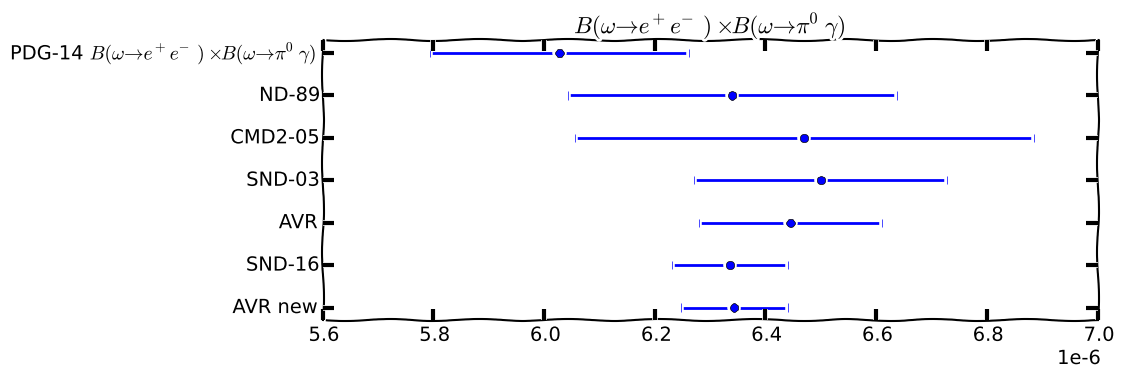
\includegraphics[width=.85\textwidth]{{img/Bw2ee_x_Bwpi0g}.png}
    \caption{$B(\omega \to e^+e^-) \times B(\omega \to \pi^0\gamma)$.
    PDG-14 --- \cite{Agashe:2014kda},
    ND-89 --- \cite{Dolinsky:1988zy},
    CMD2-05 --- \cite{Akhmetshin:2004gw},
    SND-03 --- \cite{Achasov:2003ed},
    AVR --- среднее \cite{Dolinsky:1988zy, Akhmetshin:2004gw, Achasov:2003ed},
    SND-16 --- \cite{Achasov:2016bfr},
    AVR new --- среднее \cite{Dolinsky:1988zy, Akhmetshin:2004gw, Achasov:2016bfr}}
    \label{fig:BweeXBwpig}
\end{figure}
Эта разница вызвана существованием противоречием между измереными значениями
$B( \omega \to \pi^0 \gamma ) \times B(\omega \to e^+ e^-)$,
$B( \omega \to \pi^0 \gamma ) \times B (\omega \to \pi^+ \pi^- \pi^0)$ и
$B( \omega \to \pi^0 \gamma ) / B (\omega \to \pi^+ \pi^- \pi^0)$ (см. Рис.~\ref{fig:Gw2pi0g_o_Gw2pippimpi0}).
Два последних выражения известны с точностью \SI{1.6}{\percent} и \SI{1.8}{\percent} соответственно,
и определяют нынешнее значение $B( \omega \to \pi^0 \gamma )$,
приводимое ПДГ.
Для прояснения этого противоречия необходимо улучшение точности
измерения сечения $e^+e^- \to \pi^0\gamma$ в области $\omega$-резонанса.

\begin{figure}[htbp]
    \centering
    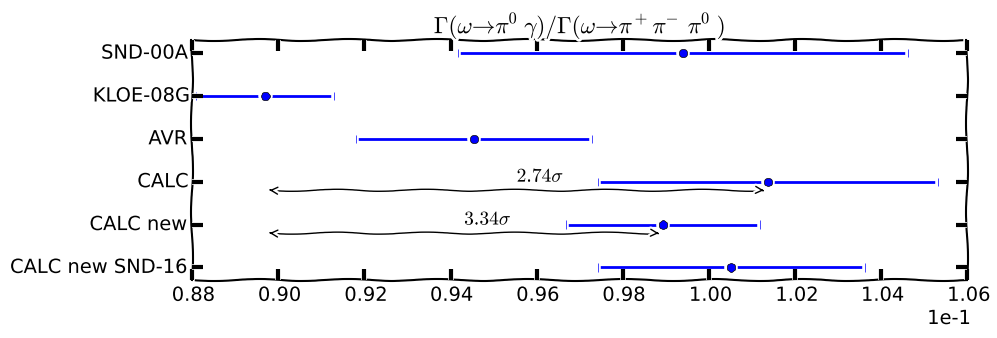
\includegraphics[width=.85\textwidth]{{img/Gw2pi0g_o_Gw2pippimpi0}.png}
    \caption{Отношение ширины распада $\omega \to \pi^0 \gamma$ к $\Gamma (\omega \to \pi^+ \pi^- \pi^0)$.
    SND-00A --- \cite{Aulchenko:2000zq},
    KLOE-08G --- \cite{Ambrosino:2008gb},
    AVR --- средние значение предыдущих двух,
    CALC --- среднее \cite{Akhmetshin:2004gw, Achasov:2003ed, Dolinsky:1988zy} делённое на среднее \cite{Akhmetshin:2003zn, Aubert:2004kj, Achasov:2003ir},
    CALC new --- среднее \cite{Akhmetshin:2004gw, Achasov:2016bfr, Dolinsky:1988zy} делённое на среднее \cite{Akhmetshin:2003zn, Aubert:2004kj, Achasov:2003ir},
    CALC new SND-16 --- \cite{Achasov:2016bfr} делённое на среднее \cite{Akhmetshin:2003zn, Aubert:2004kj, Achasov:2003ir}}
    \label{fig:Gw2pi0g_o_Gw2pippimpi0}
\end{figure}

\subsubsection{\texorpdfstring{$\rho \to \pi^0 \gamma$}{rho --> pi0 gamma}}
\label{rho-to-pi0-gamma}

Точность измерения относительной вероятности распада
$\rho \to \pi^0 \gamma$ составляет \SI{13}{\percent} и определяется статистикой
существующих измерений.

\subsubsection{\texorpdfstring{$\phi \to \pi^0 \gamma$}{}}
\label{phi-to-pi0-gamma}

Формальная точность значения ПДГ вероятности распада
$\phi \to \pi^0 \gamma$ лучше \SI{5}{\percent}.
Оно получено путём усреднения измерений \cite{Achasov:2000zd,Akhmetshin:2004gw} с систематической
ошибкой порядка \SI{8}{\percent} каждое.
Систематическая ошибка возникает из
неопределённости интерференции нерезонансной амплитуды с амплитудой
$\phi \to \pi^0 \gamma$ распада. Нерезонансная амплитуда определяется
вкладами хвостов резонансов $\omega$ и $\rho^0$, заодно дают вклад и
высшие возбуждения векторных мезонов.

Чтобы уменьшить неопределённость таких вкладов, необходимо улучшить
точность измерения сечения $e^+e^- \to \pi^0 \gamma$ в широком диапазоне
энергий от энергий \SI{\sim 300}{\MeVr} до \SI{2}{\GeVr}.

\subsection{Аномальный магнитный момент мюона}\label{mu-amm}

Как люди не могут забыть Герострата, сжёгшего храм Артемиды, так и физики
элементарных частиц рвутся попасть в истории кардинально изменив или
изничтожив современную парадигму науки --- Стандартную Модель. Некоторые
из них ищут Новую Физику пробуя другие области энергии и массы, кто-то
ищет новые распады, другие же могут мерить что-то очень точно и
сравнивать это с предсказаниями теории.
К последней группе относится изучение аномального магнитного момента мюона.

%%%%%%%%%%%%%%%%%%%%%%%%%%%%%%%%%%%%%%%%%%%%%%%%%%%%%%%%%%%%%%%%%%%%%%%%%%%%%%%%
\subsubsection{История}\label{g-2-history}

Экспериментальные измерения $a_\mu$ впервые было осуществлено в СЛАКе \cite{Garwin:1960zz}.
Затем последовала серия измерений в ЦЕРНе, уступившее свое место эксперементу в БНЛ.
В настоящий момент готовится два эксперимента по измерению $g_\mu-2$: в ФНАЛ \cite{Grange:2015fou} и Джей-ПАРКе \cite{Saito:2012zz}.


%%%%%%%%%%%%%%%%%%%%%%%%%%%%%%%%%%%%%%%%%%%%%%%%%%%%%%%%%%%%%%%%%%%%%%%%%%%%%%%%
\subsubsection{Вклады в \texorpdfstring{$g_\mu-2$}{muon g-2}}
\label{contribution-to-g-2}

Предсказываемый в рамках СМ аномальный магнитный момент мюона $f_\mu^{\text{SM}}$ принято представлять суммой трёх слагаемых
\begin{equation}
    a_\mu^{\text{SM}} = a_\mu^{\text{QED}} + a_\mu^{\text{EW}} + a_\mu^{\text{had}},
\end{equation}
где $a_\mu^{\text{QED}}$ --- электродинамический вклад,
$a_\mu^{\text{EW}}$ --- вклад слабых взаимодействий,
$a_\mu^{\text{had}}$ --- вклад сильных взаимодействий.

Не сомтре на то, что вклад $a_\mu^{\text{had}}$ меньше $a_\mu^{\text{QED}}$ примерно на четыре порядка,
его значение примерно в 100 раз превышает точность последного эксперимента в БНЛ.
Последние обстоятельство вместе с планируемым улучшением измерения $a_\mu$ в четыре раза
требует вычисления $a_\mu^{\text{had}}$ с относительной точностью \SIrange{1}{0.1}{\percent}.

\begin{figure}[htbp]
    \begin{minipage}[t]{0.24\textwidth}
        \centering
        \begin{tikzpicture}
        \begin{feynman}
			\vertex (a);
			\vertex [below = 1cm of a] (b);
			\vertex [below left = 18.8562mm of b] (c1);
			\vertex [below right = 18.8562mm of b] (c2);
			\vertex [below left = 28.2843mm of b] (d1);
			\vertex [below right = 28.2843mm of b] (d2);
			\vertex [below right = 0mm of d1] {$\mu$};
			\vertex [below left = 0mm of d2] {$\mu$};
			% \node [below = of d1] {$\mu$};
			\vertex [right = 9.3333mm of c1, blob] (c3) {};
			% \vertex [right = 8mm of c3] (c4);
			\vertex [below right = 0mm of a] {$\gamma$};
		    
		    \diagram* [small] {
			    (a) -- [photon] (b),
			    (d1) -- [fermion] (c1) -- [fermion] (b) -- [fermion] (c2) -- [fermion] (d2),
		    	(c1) -- [photon] (c3) -- [photon] (c2),
		    	% (c4) -- [photon] (c2),
		 	};
		\end{feynman}
		\end{tikzpicture}
        \caption{Ведущий адронный вклад в $a_\mu$.}\label{diag:hvp}
    \end{minipage}
    \hfill
    \begin{minipage}[t]{0.24\textwidth}
        \centering
        \begin{tikzpicture}
		\begin{feynman}
			\vertex (a);
			\vertex [below = 1cm of a] (b);
			\vertex [below left = 18.8562mm of b] (c1);
			\vertex [below right = 18.8562mm of b] (c2);
			\vertex [below left = 28.2843mm of b] (d1);
			\vertex [below right = 28.2843mm of b] (d2);
			\vertex [right = 7.3333mm of c1, dot, blue] (c3) {};
			\vertex [right = 12mm of c3, dot, blue] (c4) {};
			\vertex [below right = 0mm of d1] {$\mu$};
			\vertex [below left = 0mm of d2] {$\mu$};
			\vertex [below right = 0mm of a] {$\gamma$};
		    
		    \diagram* [small] {
			    (a) -- [photon] (b),
			    (d1) -- [fermion] (c1) -- [fermion] (b) -- [fermion] (c2) -- [fermion] (d2),
		    	(c1) -- [photon] (c3),
		    	(c4) -- [photon] (c2),
		    	(c3) -- [photon, half left] (c4) -- [scalar, blue, very thick, half left, edge label={\(\pi^{0}\), \(\eta\)}] (c3),
		 	};
		\end{feynman}
		\end{tikzpicture}
        \caption{Ведущий адронный вклад в $a_\mu$ связанный с $e^+ e^- \to ( \pi^0, \, \eta ) \gamma$.}\label{diag:hvp_Pg}
    \end{minipage}
    \hfill
    \begin{minipage}[t]{0.24\textwidth}
        \centering
        \begin{tikzpicture}
		\begin{feynman}
			\vertex (a);
			\vertex [below = 7mm of a, blob] (a1) {};
			\vertex [below = 1cm of a] (b);
			% \vertex [below = 7mm of a, blob] (a1) {};
			\vertex [below left = 17.2132mm of b] (c1);
			\vertex [below left = 4mm of b] (b1);
			\vertex [below = 4mm of b] (b2);
			\vertex [below right = 4mm of b] (b3);
			% \vertex [below = 11mm of b] (c2);
			% \vertex [right = 15mm of c1] (c2);
			\vertex [below = 12mm of b] (c2);
			\vertex [below right = 17.2132mm of b] (c3);
			\vertex [below left = 7.0711mm of c1] (d1);
			\vertex [below right = 7.0711mm of c3] (d2);
			\vertex [below right = 0mm of d1] {$\mu$};
			\vertex [below left = 0mm of d2] {$\mu$};
			\vertex [below right = 0mm of a] {$\gamma$};
		    
		    \diagram* [small] {
			    (a) -- [photon] (a1),
			    (b1) -- [photon] (c1),
			    (b3) -- [photon] (c3),
			    (d1) -- [fermion] (c1) -- [fermion] (c2) -- [fermion] (c3) -- [fermion] (d2),
			    (b2) -- [photon] (c2),
		 	};
		\end{feynman}
		\end{tikzpicture}
        \caption{Ведущий адронный вклад света на свете в $a_\mu$.}\label{diag:lbl}
    \end{minipage}
    \hfill
    \begin{minipage}[t]{0.24\textwidth}
        \centering
        \begin{tikzpicture}
		\begin{feynman}
			\vertex (a);
			\vertex [below = 1cm of a, dot, blue] (b) {};
			\vertex [below left = 10.6066mm of b, dot, blue] (c) {};
			\vertex [below left = 10.6066mm of c] (d1);
			\vertex [right = 15mm of d1] (d2);
			\vertex [below right = 21.2132mm of b] (d3);
			\vertex [below left = 28.2843mm of b] (e1);
			\vertex [below right = 28.2843mm of b] (e2);
			\vertex [below right = 0mm of e1] {$\mu$};
			\vertex [below left = 0mm of e2] {$\mu$};
			\vertex [below right = 0mm of a] {$\gamma$};
					    
		    \diagram* [small] {
			    (a) -- [photon] (b),
			    (b) -- [scalar, very thick, blue, edge label'={\(\pi^{0}\), \(\eta\)}] (c),
			    (c) -- [photon] (d1),
			    (c) -- [photon] (d2),
			    (b) -- [photon] (d3),
			    (e1) -- [fermion] (d1) -- [fermion] (d2) -- [fermion] (d3) -- [fermion] (e2),
		 	};
		\end{feynman}
		\end{tikzpicture}
        \caption{Ведущий адронный вклад света на свете в $a_\mu$ связанный с $e^+ e^- \to ( \pi^0, \, \eta ) \gamma$.}\label{diag:lbl_Pg}
    \end{minipage}
\end{figure}
В свою очередь во вкладе сильных взаимодействий принято выделять три слагаемых:
рассеяние света на свете $a_\mu^{\text{had, LbL}}$ (диаграмма~\ref{diag:lbl}),
вклады первого $a_\mu^{\text{had, LO}}$ (диаграмма~\ref{diag:hvp}) и второго $a_\mu^{\text{had, NLO}}$ порядков:
\begin{equation}
    a_\mu^{\text{had}}
    =
    a_\mu^{\text{had, LO}}
    +
    a_\mu^{\text{had, NLO}}
    +
    a_\mu^{\text{had, LbL}}.
\end{equation}

В то время как вычисление вкладов $a_\mu^{\text{QED}}$ и $a_\mu^{\text{EW}}$ успешно происходит с использованием теории возмущений ввиду малости соответствующих констант связи,
вклад сильных взаимодействий трубует иного подхода в области характерных передач импульса меньше \SI{2}{\GeVr}.
Ведущий вклад $a_\mu^{\text{had, LO}}$ рассчитывается и использованием дисперсионного соотношения
\cite{Bouchiat1961, Durand:1962zzb, Kinoshita:1967txv, Gourdin:1969dm},
позволяющего использовать экспериментальные данные \cite{Jegerlehner:2017gek}.
\begin{equation}
   	a_\mu^{\text{had}} =
   	\left( \frac{\alpha m_\mu}{3 \pi} \right)^2
   	\left(
   		\int_{{m_{\pi^0}}^2}^{{E_{\text{cut}}}^2} \dif s
   		\frac{ R_{\text{had}}^{\text{data}}(s) \hat{K}(s) }{ s^2 }
   		+
   		\int_{{E_{\text{cut}}}^2}^{\infty} \dif s
   		\frac{ R_{\text{had}}^{\text{pQCD}}(s) \hat{K}(s) }{ s^2 }
   	\right) ,
\end{equation}
где
$ m_\mu $ --- масса мюона;
$ m_{\pi^0}$ --- масса нейтрального пиона;
$ E_{\text{cut}} $ --- энергия перехода от использование вычислений на основе экспериментальных данных к результатам полученным в рамках пертрубативной КХД;
интегрирование идёт по квадрату энергии системы $s$;
$ R_{\text{had}}^{\text{data}}(s) $ и $ R_{\text{had}}^{\text{pQCD}}(s) $ --- $R$-отношение вычисленное по экспериментальным данным и согласно КХД, соответственно:
\begin{equation}
	R_{\text{had}} (s) =
   	\sigma(e^+ e^- \to \text{hadrons})
  	/
  	\frac{4 \pi \alpha(s)}{3 s} .
\end{equation}
Ядро интегрирования $\hat{K}(s)$ определено следующим образом
\begin{equation}
	\hat{K}
  	=
   	\frac{3 s}{{m_\mu}^2}
  	\int_0^1 \dif x
  	\frac{ x^2 (1-x) }{ x^2 + \frac{s}{{m_\mu}^2} (1-x) } .
\end{equation}

Таким образом,
вклад изучаемых процессов в лидирующий влад адронной поляризации вакуума можно представить диаграммой~\ref{diag:hvp_Pg}.

Расчёт вклада света на свете представляет наибольшую сложность,
так как он не поддаётся вычислениям ни в рамках теории возмущений КХД,
ни связыванию с экспериментальными данными использую дисперсионное соотношение.
Производимые расчёты оказываются модельно зависимы,
приводя к сравнительно большой неопределённости вычислений.
Адронный блок диаграммы~\ref{diag:lbl} представляется в виде обемена адронами.
Доминирующий вклад вносят псевдоскалярные мезоны $\pi^0$, $\eta$, $\eta^\prime$,
при этом процесс выгляит как на диаграмме~\ref{diag:lbl_Pg}.
Развитие моделей,
фиксирование их свободных параметров и проверка,
разумеется связано с использованием экспериментальных данных.
Косательно псевдоскалярных мезонов $P$ особенно ценными является измерение форм-фактора
$F_P ( {q_1}^2, \, {q_2}^2 )$.
Однако, полезными также являются и вся остальная достпуная информация,
в том числе сечение реакция типа $e^+ e^- \to P \gamma$.


%%%%%%%%%%%%%%%%%%%%%%%%%%%%%%%%%%%%%%%%%%%%%%%%%%%%%%%%%%%%%%%%%%%%%%%%%%%%%%%%
\subsubsection{Расчёт вкладов в различных моделях}
\label{contribution-calculation}


Как было сказано выше,
невозможность прямого вычисления $a_\mu^{\text{had, LO}}$
в теории сильных взаимодействий обойдена при помощи дисперсионно соотношения,
требущего в свою очередь знания зависимости сечений процессов
$e^+ e^- \to \gamma^* \to \text{hadrons}$
от энергии в системе центра масс $\sqrt{s}$.
Последнее важно как для инклюзивного,
так и для эксклюзивного вычисления $R_{\text{had}}^{\text{data}}$.
В виду того,
что экспериметальные данные доступны в конретных точках или диапазонах по энергии,
и иногда могут и отсутсвовать вовсе или их точность неудовлетворительна,
а в то же время для других каналов и энергий наблюдается перекрытие,
требуется производить аппроксимацию или усреднение.
Ниже будет упомянуто о различных методиках решения задачи вычисления $R_{\text{had}}^{\text{data}}$,
приминительно к вкладам процессов $\pi^0 \gamma$ и $\eta \gamma$.


%%%%%%%%%%%%%%%%%%%%%%%%%%%%%%%%%%%%%%%%%%%%%%%%%%%%%%%%%%%%%%%%%%%%%%%%%%%%%%%%
% KNT18
В статье \cite{KNT18} экспериментальные данные разбиваются на кластеры.
Внутри кластера идёт поиск центра тяжести и его ошибки путём иттерационной минимизации $\chi^2$ сечения
представленного ломанной кривой, соединяющий центры кластеров.
Таким образом дальнейшее интгрирование в том же линейном приближении является оптимпальным вариантом вычисления вкладов в $a_\mu^{\text{had, LO}}$.
Полученные результаты касательно процессов $\pi^0 \gamma$ и $\eta \gamma$ приведены в таблицах~\ref{tab:amm_pi0g}, \ref{tab:amm_etag}.
%%%%%%%%%%%%%%%%%%%%%%%%%%%%%%%%%%%%%%%%%%%%%%%%%%%%%%%%%%%%%%%%%%%%%%%%%%%%%%%%

\begin{table}
	\centering
	\caption{Вклад в $a_\mu^{\text{had, LO}}$ и $\Delta \alpha_{\text{had}} ({M_Z}^2) $ процесса 
		$e^+ e^- \to \pi^0 \gamma$.}\label{tab:amm_pi0g}
	\begin{tabular}{ccccc}
		Энергия, \si{\GeVr} & $a_\mu^{\text{had, LO}}$ & $\Delta \alpha_{\text{had}} ({M_Z}^2) $ & Источник \\
		\hline
		$[m_\pi , \, 0.6]$ & \num{0.12 \pm 0.01} & \num{0.00 \pm 0.00} & \cite{KNT18} \\
		$[0.6 , \, 1.350]$ & \num{4.46 \pm 0.10} & \num{0.36 \pm 0.01} & \cite{KNT18} \\
		$[m_\pi , \, 1.8]$ & $4.29 \pm 0.06 \pm 0.04 \pm 0.07$ & $0.35 \pm 0.00 \pm 0.00 \pm 0.01$ & \cite{Davier:2017zfy} \\
		$[0.318 , \, 2]$ & \num{4.06 \pm 0.16} & \num{0.35 \pm 0.01} & \cite{Jegerlehner:2017gek} \\
		$[m_\pi , \, 0.6]$ & \num{0.13 \pm 0.01} &  & \cite{Ahmadov:2010hq} \\
		$[0.6 , \, 1.03]$ & \num{4.5 \pm 0.15} &  & \cite{Ahmadov:2010hq}
	\end{tabular}
\end{table}

\begin{table}
	\centering
	\caption{Вклад в $a_\mu^{\text{had, LO}}$ и $\Delta \alpha_{\text{had}} ({M_Z}^2) $ процесса 
		$e^+ e^- \to \eta \gamma$.}\label{tab:amm_etag}
	\begin{tabular}{cccc}
		Энергия, \si{\GeVr} & $a_\mu^{\text{had, LO}}$ & $\Delta \alpha_{\text{had}} ({M_Z}^2) $ & Источник \\
		\hline
		$[m_\eta , \, 0.66]$ & \num{0.12 \pm 0.01} & \num{0.00 \pm 0.00} & \cite{KNT18} \\
		$[0.66 , \, 1.35]$ & \num{4.46 \pm 0.10} & \num{0.36 \pm 0.01} & \cite{KNT18} \\
		$[m_\eta , \, 1.8]$ & $0.65 \pm 0.02 \pm 0.01 \pm 0.01$ & $0.08 \pm 0.00 \pm 0.00 \pm 0.00$ & \cite{Davier:2017zfy} \\
		$[0.318 , \, 2]$ & \num{0.56 \pm 0.02} & \num{0.06 \pm 0.00} & \cite{Jegerlehner:2017gek} \\
		$[0.69 , \, 1.33]$ & \num{0.73 \pm 0.03} &  & \cite{Ahmadov:2010hq}
	\end{tabular}
\end{table}

%%%%%%%%%%%%%%%%%%%%%%%%%%%%%%%%%%%%%%%%%%%%%%%%%%%%%%%%%%%%%%%%%%%%%%%%%%%%%%%%
% DHMZ17
Авторы работы \cite{Davier:2017zfy} для вычисления вкладов проводят квадратичную интерполяцию экспериментальных данных для каждого канала каждого анализа.
Полученное приблежение используют для вычисления сечений в бинах шириной \SI{1}{\MeVr}.
Далее в каждом бине каждого канала идёт усреднение по всем измерением.
В случае противоречивости данных ошибка их комбинации масштабируется.
%%%%%%%%%%%%%%%%%%%%%%%%%%%%%%%%%%%%%%%%%%%%%%%%%%%%%%%%%%%%%%%%%%%%%%%%%%%%%%%%

%%%%%%%%%%%%%%%%%%%%%%%%%%%%%%%%%%%%%%%%%%%%%%%%%%%%%%%%%%%%%%%%%%%%%%%%%%%%%%%%
% FJ17
% BDDJ12&17
В работах \cite{Benayoun:2016krn, Jegerlehner:2017gek}
расчёт вкладов в АПВ идёт на основе комбинации модели доминантности векторных мезонов
с моделью нарушения скрытой локальной симметрии.
Полученной комбинацией идёт подгонка экспериментальных данных сразу в нескольких каналах $e^+ e^-$-аннигиляции
и спектральных функций $\tau$-лептона.
%%%%%%%%%%%%%%%%%%%%%%%%%%%%%%%%%%%%%%%%%%%%%%%%%%%%%%%%%%%%%%%%%%%%%%%%%%%%%%%%

%%%%%%%%%%%%%%%%%%%%%%%%%%%%%%%%%%%%%%%%%%%%%%%%%%%%%%%%%%%%%%%%%%%%%%%%%%%%%%%%
% AKV10
В статье \cite{Ahmadov:2010hq}
используется расширенная модель Намбу--Иона-Лазинио,
для определения параметров которой происходит подгонка экспериментальных данных,
а затем вычисление вкладов в $a_\mu^{\text{had, LO}}$.
%%%%%%%%%%%%%%%%%%%%%%%%%%%%%%%%%%%%%%%%%%%%%%%%%%%%%%%%%%%%%%%%%%%%%%%%%%%%%%%%



\subsection{Структура мезонов}
\label{meson-structures}

Являясь частью СМ квантовая хромодинамика отвечает за процессы с участием адронов. Однако, она весьма ограничена в использовании для области энергий с характерной передачей импульса ниже \SI{1}{\GeVr}.
Это привело к популярности феноменологических подходов к описанию физики в данной области энергий.
Используемые модели обладают рядом свободных параметров,
которые можно фиксировать из экспериментальных данных.
С другой стороны,
такие модели не только подгоняют уже имеющиеся данные,
но обладают предсказательной силой,
величину которой хорошо бы проверять не только качественно,
но и числено.
Для двух этих целей --- определение свободных параметров и проверка верности ---
прекрасно подходят сечения изучаемых процессов.
Оба они относятся к магнитным радиационным переходам М1,
что делает их хорошим инструментом для изучения структуры мезонов в свете различных феноменологических моделей,
например кварковой модели с $SU(3)$ или даже с $SU(6)$ симметрией.

\resizebox{.3\paperwidth}{!}{%
\begin{tikzpicture}
	\begin{feynman}
		%\vertex (a) {\(e^{-}\)};
		%\vertex [below right=of a] (b);
		%\vertex [below left=of b] (c) {\(e^{+}\)};
		\vertex (b);
		\vertex [above left=of b] (a) {\(e^{-}\)};
		\vertex [below left=of b] (c) {\(e^{+}\)};
		\vertex [right=of b, dot, blue] (d) {};
		\vertex [above right=of d] (f1) {\(\gamma\)};
	    \vertex [below right=of d, dot, blue] (m1) {};
	    \vertex [above right=of m1] (f2) {\(\gamma\)};
	    \vertex [below right=of m1] (f3) {\(\gamma\)};
		    
	    \diagram* [small] {
		    (a) -- [fermion] (b) -- [fermion] (c),
		    (b) -- [photon, edge label=\(\gamma^{*}\)] (d) [blob],
		    (d) -- [photon] (f1),
		    (d) -- [scalar, blue, very thick, edge label'={\(\pi^{0}\), \(\eta\), (\(\eta^\prime\))}] (m1),
		    (f3) -- [photon] (m1) [blob] -- [photon] (f2),
			% (m1) -- [photon] (f3),
	 	};
	\end{feynman}
\end{tikzpicture}
}

Особый интерес представляют структуры мезонов $\eta$ и $\eta^\prime$, так как в них допускается наличия вкладов $c\bar{c}$-кварков или примесь глюонов. 

В своей статье О'Доннелл \cite{ODonnell:1981sj} исследует кварковый состав мезонов в
рамках кварковой модели и проверяет получаемые результаты с помощью
экспериментальных данных, в то числе, по магнитнодипольным переходам
векторных мезонов в пару фотон-псевдоскаляр.

%В статье Болла, Фрере, Титгэт \cite{Ball:1995zv} ках феноменологической модели.% что за модель?
%С этой целью рассматриваются радиационные распады
%$P \to \gamma \gamma$, $V \to P \gamma$ и $P \to V \gamma$. Упор
%делается на работу с основными состояниями, таким образом не учитываются
%вклады возбуждённых состояний лёгких векторных мезонов.

Эскрибано и Надаль \cite{Escribano:2007cd} исследовали вклад в глюонов в состояния $\eta$
и $\eta(958)$ провядя феноменологический анализ радиационных распадов
$V (P) \to P (V) \gamma$ в рамках нарушенной SU(3) с учётом
пространственного перекрытия волновых функций $| V \rangle$ и
$|P \rangle$. Авторы заключают, что глюонная составляющая в $\eta$ и
$\eta(958)$ пренебрежимо мала, угол смешивание
$\eta-\eta^\prime = \ang{41.4 \pm 1.3}$, и подчёркивают важность
экспериментальных данных по $(\rho, \, \omega, \, \phi ) \to \eta \gamma$ для
проведённых вычислений.

В статье Бенаёун, ДельБуоно, Эйдельмана, Иванченко и О'Коннелла \cite{Benayoun:1999fv} даётся разбор
вопроса о совместном согласованном описании радиационных и лептонных
распадов лёгких мезонов ($V(P) \to P(V)\gamma$, $P \to \gamma \gamma$ и
$V \to e^+ e^-$).


\subsection{Другие измерения}\label{other-measurments}

Данные измерения не будут являться первыми, однако,
они возможно смогут претендовать на сравнимые или улучшенные точности в уже исследованных областях энергии $\sqrt{s}$
или быть даже первыми и одними из первых в других.
Ниже приведены данные о предыдущих измерениях с целью выявления современной ситуации в этой области извлечения данных природы.
Наиболее значимые результаты измерений приведены на рисунке~\ref{fig:cs_pi0g_prev} для процесса $e^+ e^- \to \pi^0 \gamma$
и на рисунке~\ref{fig:cs_etag_prev} для $e^+ e^- \to \eta \gamma$.

\begin{figure}[htbp]
	\begin{minipage}[T]{.48\textwidth}
		\centering
		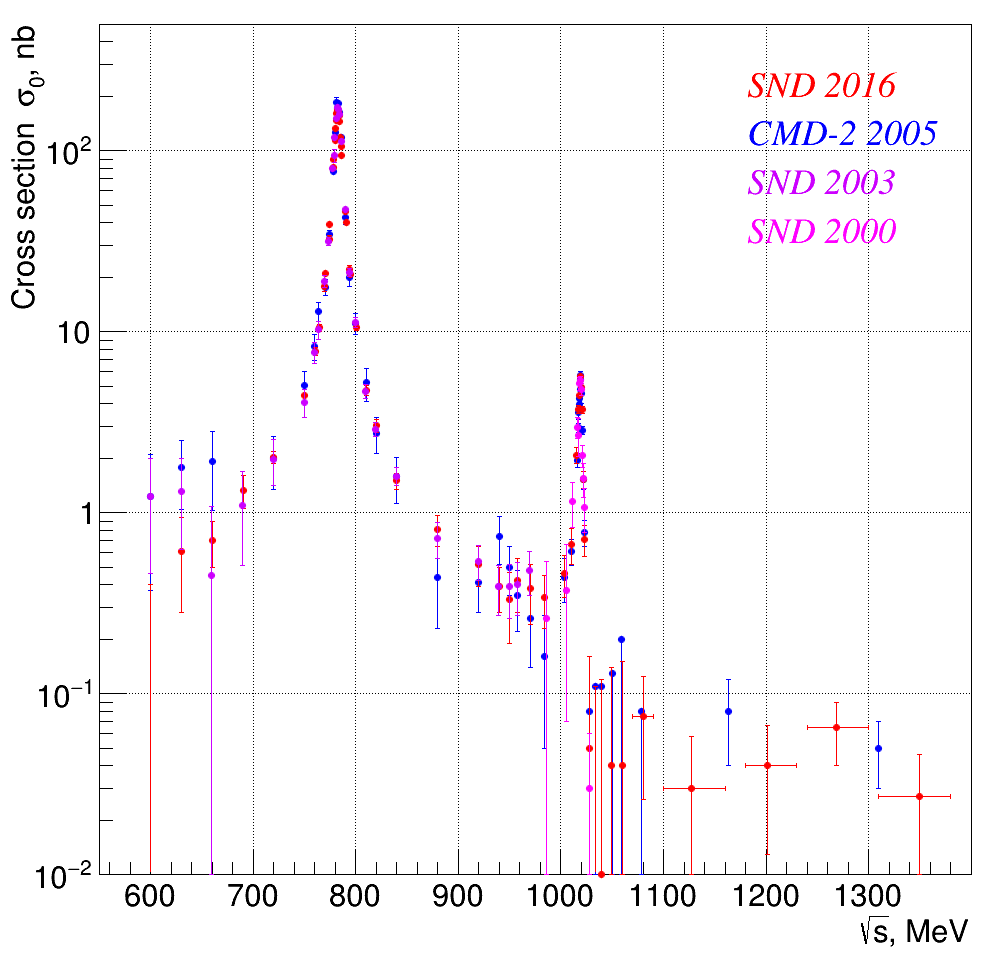
\includegraphics[width=\textwidth]{img/cs_pi0g_550_1400.png}
		\caption{Некоторые предыдущие измерения сечения $e^+ e^- \to \pi^0 \gamma$.}\label{fig:cs_pi0g_prev}
	\end{minipage}
	\hfill
	\begin{minipage}[T]{.48\textwidth}
		\centering
		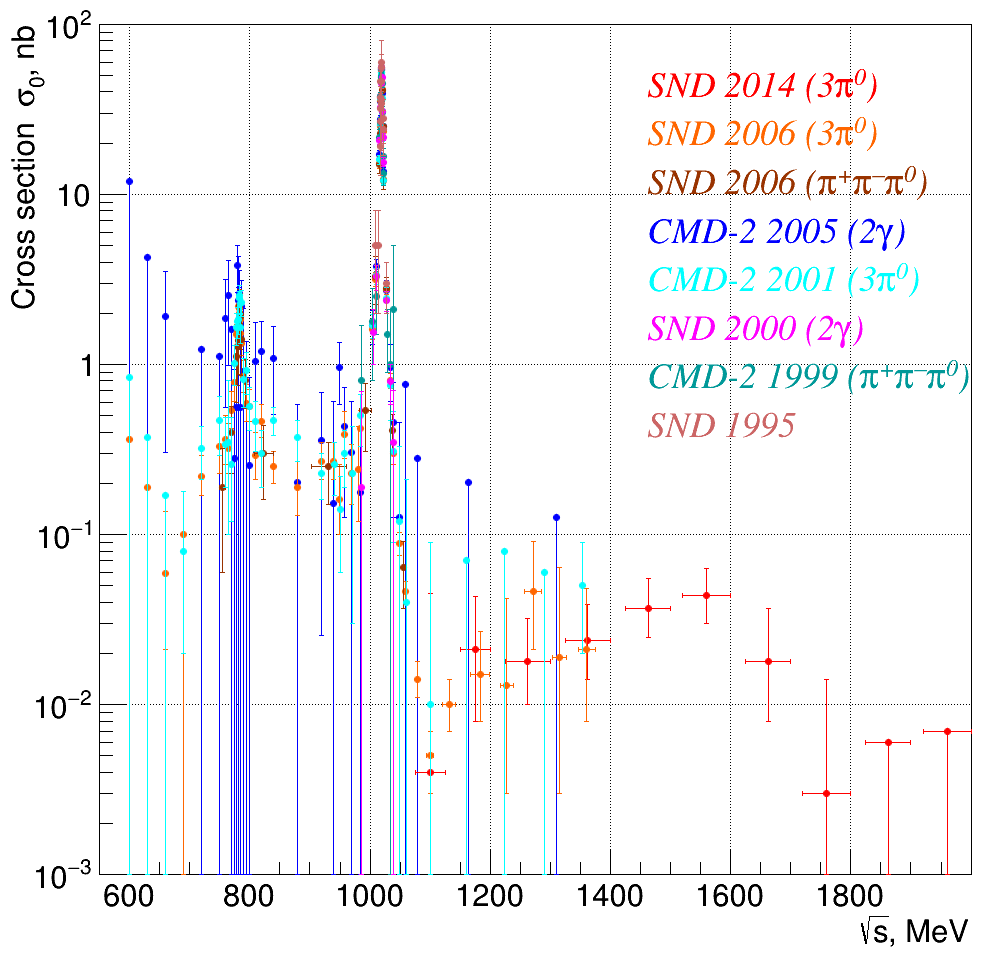
\includegraphics[width=\textwidth]{img/cs_etag_550_2000.png}
		\caption{Некоторые предыдущие измерения сечения $e^+ e^- \to \eta \gamma$.}\label{fig:cs_etag_prev}
	\end{minipage}
\end{figure}

Сечение процесса $e^+e^-\to\eta\gamma$ исследовалось во многих экспериментах.
Первые опубликованные данные появились в 1976 году из Орсая \cite{Cosme:1975rs}.
Дальнейший поток данных в основном происходит из установок Новосибирска, начиная с работы выполненной на детекторе НД \cite{Druzhinin:1984zq} и продолжая данными с КМД-2 \cite{Akhmetshin:1995vz, Akhmetshin:1999zv, Akhmetshin:2001hm, Akhmetshin:2004gw} и СНД \cite{Achasov:1997nq, Achasov:2000zd, Achasov:2006dv, Achasov:2013eli}.
Также известно измерение сечения реакции на детекторе BaBar \cite{Aubert:2006cy}.

Сечение процесса $e^+e^-\to\pi^0\gamma$ измерено несколько раз, начиная с работы в Орсаи \cite{Cosme:1975rs} и продолжая работами в Новосибирске \cite{Druzhinin:1984zq, Achasov:2000zd, Achasov:2003ed, Akhmetshin:2004gw, Achasov:2016bfr}.



\subsection{Отбор событий}

Отбор разбивается на несколько шагов. В начале пути отбираются полностью нейтральные события с тремя и более фотонами.
Причём от каждого фотона требуется, чтобы его энергия была больше \SI{30}{\MeVr} и полярный угол не тяготеет к вакуумной трубе.
Для таких событий вычисляется полная энергия $E_{\text{tot}}$ и импульс $P_{\text{tot}}$ системы частиц.
Характерное распределение представлено на рисунке~\ref{fig:EtvsPt5095}.
Сгущение событий около точки $P_{\text{tot}} = \SI{0}{\MeVr}$ и $E_{\text{tot}} = \sqrt{s}$ отвечаем искомым событием.
От этой группы тянется два хвоста под углами \ang{45} вверх и вниз.
Равное отколонение импульса $|P_{\text{tot}} - \SI{0}{\MeVr}|$ и энергии $|E_{\text{tot}} - \sqrt{s}|$
---
указание на то,
что данная девиация вызвана одной частицей.
Хвост уходящий вверх соответствует учёту излишней энергии в системе,
как правило такое соответствует тому,
что фотонным кластерам приписывается излишнее энерговыделение или имеется дополнительный кластер не возникший в следствие $e^+e^-$-аннигиляции,
к которой относится конкретное событие.
Хвост уходящий вниз, наоборот свидетельствует о недостатке энергии-импульса в системе.

\begin{figure}
	\centering
	\label{fig:EtvsPt5095}
	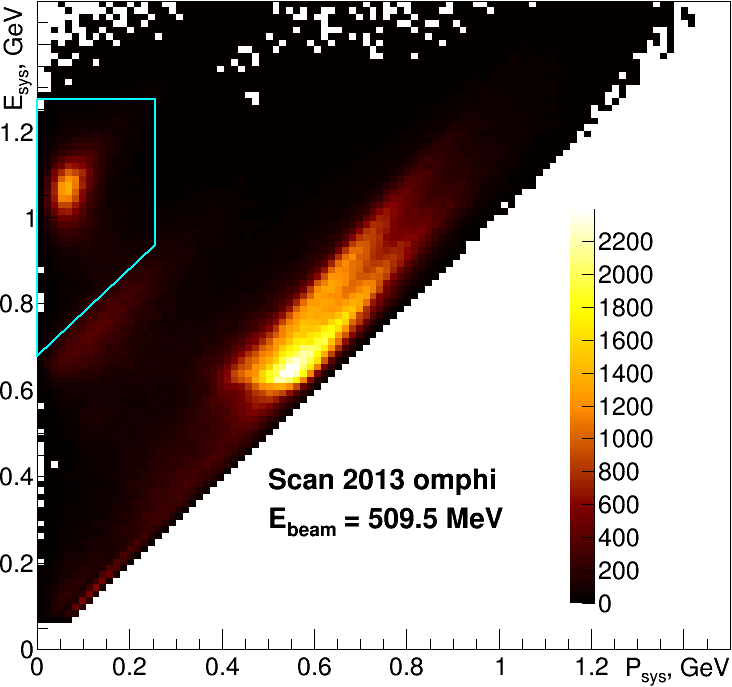
\includegraphics[width=.5\textwidth]{img/EtvsPt5095.png}
	\caption{Зависимость полной энергии события $E_{\text{tot}}$ от модуля полного импульса $P_{\text{tot}}$.
		Данные эксперимета, сезон 2013 $\omega \ \phi$, $E_{\text{beam}} = \SI{509.5}{\MeVr}$.
		Циановой линией обозначены условия отбора.}
\end{figure}

Теперь наступает шаг по отбору событий, в которых импульс системы близок к нулю,
а энергии к удвоенной энергии пучков.
Такой отбор направлен на те события,
где детектор зарегистрировал все частицы конечного состояния,
в то время как дополнительные кластеры в калориметре не дают значительного вклада.

На следующим шаге проводится кинематическая реконструкция событий.
В неё заложены законы сохранения энергии-импульса системы в целом и общая точка вылета фотонов.
Наличие промежуточных состояний $\pi^0$ или $\eta$ не требуется,
так как это оставляет крайне мало параметров последующей селекции сигнальных событий от фотона.
Если в событие присутствует более трёх фотонов,
то кинематическая реконструкция проводится для каждой возможной тройки и оставляется та,
что имеет наименьший $\chi^2$.
Подробнее о процедуре кинематической реконструкции изложено в разделе~\ref{sec:kf}.

Теперь, 
когда составлен набор трёхчастичных событий, 
отбрасываются все события, 
в которых не один из фотонов не полетел в центральную часть калориметра, 
а именно в систему \ce{LXe}. 
Такое условие предполагает наличие точки конверсии фотона,
определённой по полосковой электронике \ce{LXe} с хорошим координатным разрешением.

На этом отбор кандидатов закончен. 
В дальнейшем они разделяются на две большие пересекающиеся подгруппы: 
хотя бы один фотон попал в \ce{LXe} и все фотоны попали в центральную часть калориметра.
Попадание в центральную часть определяется по полярному углу фотона до кинематической реконструкции как $0.9 < \theta < \pi - 0.9$.



\subsubsection{Кинематическая реконструкция}
\label{sec:kf}

В ходе физической реконструкции событий закладывается гипотеза о знании точки вылета фотонов.
Предполагая угол влёта фотона в калориметр,
реконструируется его энергия по зарегистрированному энерговыделению.
Для нейтральных событий точка взаимодействия начальных лептонов не определена вдоль их движения и,
как следствие,
делается предположение о их вылете из центральной плоскости детектора $z = 0$.
Естественно,
это ухудшает разрешение параметров фотонов.
С целью преодоления такого недостатка проводится кинематическая реконструкция событий,
приводящая к улучшению ситуации,
что особенно ярко проявляется на распределениях инвариантных масс фотонов,
отвечающих мезонам.

Алгоритм кинематической реконструкции был разработан на основе работ \cite{Bukin2003-27, Bukin2005-51, Bukin2008-3}.
В них были описаны несколько подходов к составлению и минимизации функционалов.
Выбор остановился на составлении функционала со штрафными функциями,
сила которых регулируется весовыми коэффициентами
---
множителями Лагранжа.
Саму минимизацию было решено проводить численным методом.

В основу кинематической реконструкции заложены законы сохранения энергии-импульса системы в предположении общей точки вылета фотонов.

От энергии фотонов требуется, чтобы их сумма была равна сумме энергий пучков в системе центра масс. Последняя, в лучшем случае измерена с использованием обратного комптоновского рассеяния фотонов лазера на пучке. Следующая по приоритету информации энергии происходит из параметров частиц в различных физических процессах. Наихудший вариант --- уставная энергия ВЭПП-2000. Полный импульс системы полагается равными нулю. Эти два условия в купе говорят об отсутствие рассмотрения радиационного излучения как начальных, так и конечных частиц.
Логичным шагом развития кинематической реконструкции было бы добавления возможности уноса энергии и импульса вдоль оси пучков --- оси $z$.

Общая точка вылета определяется тремя координатами, две из которых фиксированы --- $x$ и $y$ берутся из дерева \textit{tr\_ph} для каждого захода (данный параметры усредняются по всем событиям в заходе с трековыми центральными вершинами в предположении стабильности орбиты пучков).
Разумеется, эти два параметра можно было бы отпустить, но их разрешение несравненно больше, чем у всех остальных, потому это можно отнести к категории мало-играющих факторов в ходе минимизации, разве что они увеличат затраченное время на процесс, и пренебречь ими. 
Третья координата $z$ точки взаимодействия свободна от каких-либо условий, другими словами, её разрешение бесконечно плохое и она не даёт вклада в $\chi^2$.

Когда говорят о координатах фотонов, подразумевается точка конверсии фотона в электрон-позитронную пару, 
являющуюся началом электромагнитного ливня в веществе детектора и не только. 
Определение этой точки конверсии сильно зависит от того, в каком месте она, конверсия, произошла.
Если рассматривать калориметры КМД-3, 
то при рождении ливня в \ce{LXe} в большинстве случаев срабатывает полосковая электроника, позволяя определить координаты с точностью \SIrange[range-phrase=--]{2}{4}{\mm} (?), 
либо по башням, если нет информации с полосок, но точность падает --- глубина равняется половине глубины башни а положение на цилиндрической поверхности средневзвешенному. 
В случае попадания фотона в \ce{BGO} калориметр $r$ и $\varphi$ координаты определяются по центру тяжести энерговыделения, 
а $z$ зависит от угла попадания фотона в калориметр в предположении вылета из центра детектора. 
Когда же фотон зарегистрирован только в \ce{CsI}, то $z$ и $\varphi$ определяются по центру тяжести, 
а $r$ устанавливается равной положению ближайшей к центру грани кристалла.

Координаты конверсии каждого фотона описываются в деревьях \textit{tr\_ph} параметрами $\rho$, $\theta$ и $\varphi$.
К двум последним прилагаются их ошибки $\sigma_\theta$ и $\sigma_\varphi$.
Так как $x_0$ и $y_0$ фиксированы,
то варьирование азимутального угла фотонов корректно.
Однако,
значение полярного угла определяется по точке вылета,
в том числе неопределённой точки $z_0$,
и точке конверсии фотона в калориметре.
Другими словами,
варьирование самого угла $\theta$ двигает две точки.
Поэтому необходимо их развязать для упрощение кинематической реконструкции.
Для цилиндрической части калориметра для варьирование выбирается координата $z$ точки конверсии,
связанная с полярным углом следующим образом:
\begin{equation}
    \theta_i
    =
    \arctg
    \frac{\rho_i}{z_i + \delta z_i + z_0} .
\end{equation}
Для торцевого калориметра варьирование идёт по координате $\rho$,
связь полярного угла с которой определяется как
\begin{equation}
    \theta_i
    =
    \arctg
    \frac{\rho_i + \delta \rho_i}{z_i + z_0} .
\end{equation}

Тем самым минимизация функционала производится варьированием $3 N + 1$ параметром



\begin{equation}
F = w_L L + w_W W + w_N \left( N_1 + N_2 + N_3 \right) + w_M M.
\end{equation}
$L$ отвечает за $\chi^{2}$
\begin{equation}
	L
	= 
	\sum_{i, \, \mu} 
	\frac{ \left( p^{i}_\mu -p^{fix,\,i}_\mu \right)^2 }{{\sigma^i_\mu}^2} , 
	\, \mu = E, \theta, \phi, \, i = \gamma_1, \gamma_2, \gamma_3.
\end{equation}
$W$ представляет закон сохранения энергии
\begin{equation}
	W = \left[ \sqrt{s} - E^{\gamma_1}- E^{\gamma_2}- E^{\gamma_3} \right]^2 ,
\end{equation}
$N_i$ --- закон сохранения импульса
\begin{equation}
	N_i = \left[ p_i^{\gamma_1} + p_i^{\gamma_2} + p_i^{\gamma_3} \right]^2, \, i=x,y,z ,
\end{equation}



\subsubsection{Определение числа сигнальных событий}

Определения числа сигнальных событий происходит по распределению инвариантных масс пар фотонов,
иначе по массе отдачи одного из фотонов.
Для каждой энергии и каждого  изучаемого процесса выбирается наиболее вероятная пара фотонов,
в которую распался псевдоскалярный мезон.
Стоит помнить, что фотоны упорядоченны по энергии $E_1 > E_2 > E_3$.
Так в большой части диапазона доступных энергий для процесса $e^+ e^- \to \eta \gamma$ предпочтительна масса $m_{23}$,
а для $\pi^0 \gamma$ --- $m_{23}$.

\begin{figure}
	\begin{minipage}[T]{.48\textwidth}
		\centering
		\label{fig:cm12cal2}
		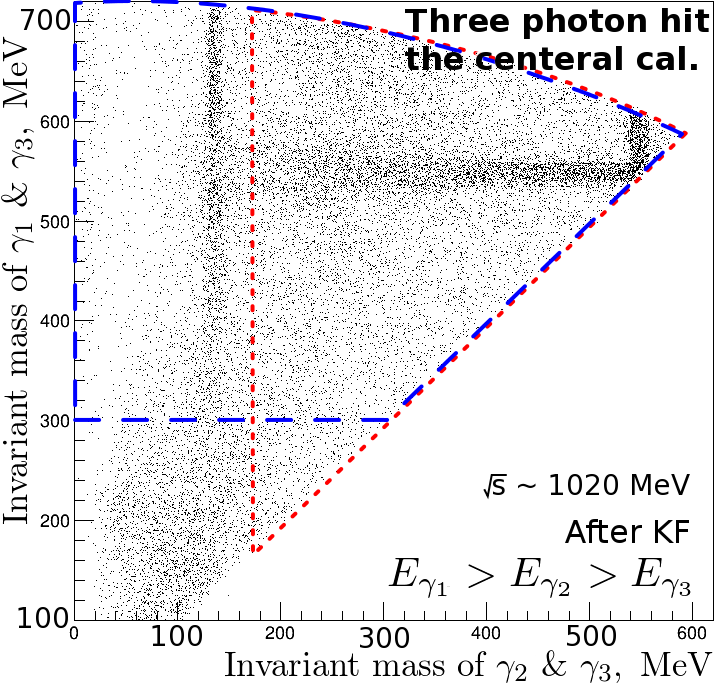
\includegraphics[width=\textwidth]{img/cm12cal2.png}
		\caption{Диаграмма Далица для событий $e^+ e^- \to 3 \gamma$ после кинематической реконструкции,
			когда все три фотона попали в \ce{LXe} калориметр.
			Данные эксперимета, сезон 2013 $\omega \ \phi$, $E_{\text{beam}} = \SI{510}{\MeVr}$.
			Синей линией обозначена кинематическая область используемая для определения числа событий $\pi^0 \gamma$,
			красная линия --- $\eta \gamma$.}
	\end{minipage}
	\hfill
	\begin{minipage}[T]{.48\textwidth}
		\centering
		\label{fig:etag}
		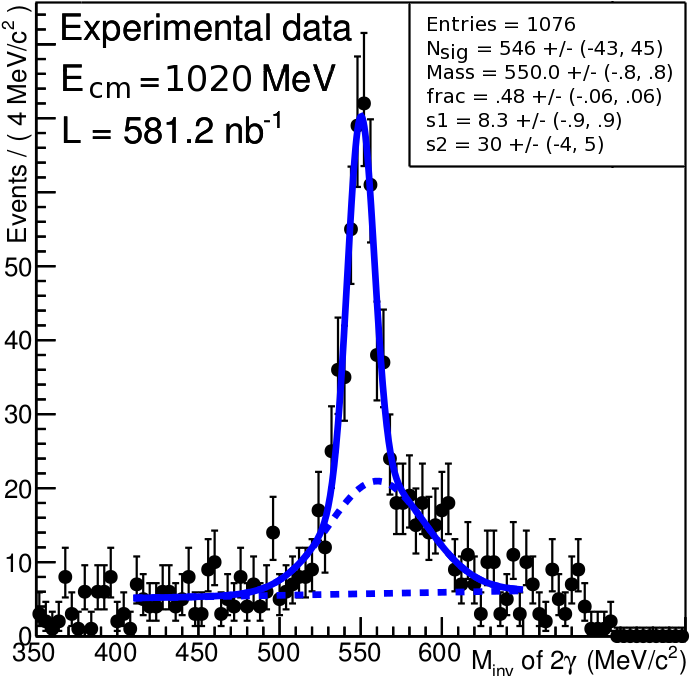
\includegraphics[width=\textwidth]{img/etag.png}
		\caption{Распределение по инвариантной массе двух фотонов после кинематической реконструкции,
			когда все три фотона попали в \ce{LXe} калориметр.
			Данные эксперимета, сезон 2013 $\omega \ \phi$, $E_{\text{beam}} = \SI{510}{\MeVr}$.
			Сплошной синей линией показана аппроксимирующая кривая $f_{\text{sig}} + f_{\text{bkg}}$.
			Синими штрихованами линиями показаны $f_{\text{bkg}}$ и сумма $f_{\text{bkg}}$ и одна составляющая $f_{\text{sig}}$.}
	\end{minipage}
\end{figure}

При построении таких распределений используется ряд дополнительных критериев на параметры частиц их системы в целом.
Минимальное число фотонов зарегистрированных в центральной части калориметра является одним из самых существенных таких отборов.
Для него используется два критерия,
либо хотя бы один фотон летит в цилиндрический калориметр,
либо все фотоны зарегистрированы в цилиндрической части.
Второй набор событий является подклассом первого.
Также второй набор аналогичен отборам проводимым при анализе на детекторе КМД-2,
что делает его более интересным для сравнения результатов.
Данный отбор даёт выбрать в пользу большей статистики или лучшего разрешения по инвариантной массе.

Вторым важным отбором является условие на минимальную энергию фотона,
как правило, она ставится равной \SI{50}{\MeVr}.
Данное число выбрано согласно моделированию и,
с одной стороны, подавляет фон в калориметре,
особенно в его торцевой части, с другой,
оказывает малое влияние на число сигнальных событий.
Таким образом возрастает отношение сигнал/фон.

Существует ещё условие на число зарегистрированных фотонов в событии.
В области $\phi$-мезона,
где сечение $e^+ e^- \to \eta \gamma$ достигает своего максимума,
это позволяет подавить вклад от канала распада $\eta \to \pi^+\pi^-\pi^0$,
ставя ограничение на число фотонов $n < 6$.

Непосредственно для определения числа сигнальных событий проводится подгонка распределения суммой сигнальной и фоновой функций.
Для описания фона используется полином.
Сигнал же описывается суммой нормальных распределений с общим нормировочным множителем.
Используемый алгоритм отбора событий также направлен на подавление фона,
что часто приводит к его малой статистике и трудности определения формы,
особенно под сигнальным пиком.
Для решения данной проблемы используется моделирование,
своё для каждой точки по энергии,
на которое опирается подгоночная функция --- так называемая одновременная подгонка (simultaneous fit).
В областях по энергии, где сечение мало,
и определение как числа событий сигнала,
так и фона затруднено привело к использованию небинированной подгонки,
которая позволяет в таких скользких ситуациях избежать проблем с выбором подходящего бинирования распределения.
Также для малой статистики вопрос, как правило,
идёт о определении верхнего предела, что, как временное решение,
приводит к определению асимметричных ошибок с помощью алгоритма Minos.


\subsection{Определение эффективности отбора}



\subsubsection{Моделирование}

\begin{figure}
	\centering
	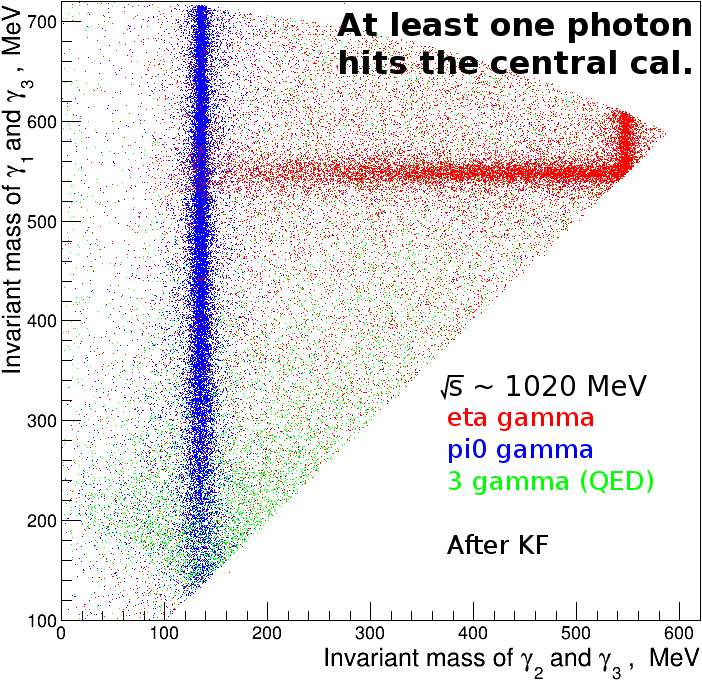
\includegraphics[width=.5\textwidth]{img/cm12mc.png}
	\caption{Диаграмма Далица после КР 
			для событий моделирования в области $\phi$-мезона
			$e^+ e^- \to \pi^0 \gamma$ (синие точки),
			$e^+ e^- \to \eta \gamma$ (красные точки)
			и трёхквантовой аннигиляции (зелёные точки),
			когда хотя бы один фотон попал в \ce{LXe} калориметр.\label{fig:cm12mc}}
\end{figure}

Для определения эффективности отбора событий $e^+ e^- \to \pi^0 \gamma, \, \eta \gamma$ по конченому трёхфотонному состоянию разработанный метод применялся к данным моделирования.
Моделирование проводилось с помощью пакета \emph{GEANT4}, \cite{geant4Allison:2006ve}.
Пример диаграммы Далица приведён на рисунке~\ref{fig:cm12mc}.
В моделирование учитывались все возможные каналы распадов псевдоскалярных мезонов, также моделирование идёт с излучением радиационных фотонов.
% На рисунках \textbf{пара рисунков с эффективностью от с.м. энергии} представлены эффективности при разных условиях отбора в зависимости от полной энергии в системе центра масс.

Падение эффективности с ростом энергии объясняется увеличением вероятности иметь маленькие углы между фотонами в событие,
что приводит к сливанию электромагнитных ливней в калориметре детектора.

Вблизи порога реакции $e^+ e^- \to \eta \gamma$ монохроматичный фотон становится мягким, что уменьшает вероятность регистрации.
Так начиная при энергии системы $\sqrt{s} = \SI{666}{\MeVr}$ энергия монохроматичного фотона равна \SI{30}{\MeVr}, что соответствует порогу на рассмотрения фотона как значащего.

% Для определения эффективности разработанного метода применялся на данных моделирования $e^+ e^- \to
% \eta \gamma$ и $e^+ e^- \to \pi^0 \gamma$.
% Причём с распадом псевдоскалярных мезон во все возможные каналы.
Так характерная эффективность в области $\phi$-мезона без ограничения на углы вылета конечных
фотонов составила \SI{23.7}{\percent} для $\eta \gamma$ процесса.
Для $\pi^0 \gamma$ при условии попадания хотя бы одного фотона в центральную часть детектора
составляет приблизительно \SI{5}{\percent},
при этом наблюдается спад эффективности с ростом $\sqrt{s}$.



\subsubsection{Поправка к эффективности регистрации фотонов}



Эффективность реконструкции фотонов в моделировании и эксперименте определено по событиям процесса
$e^+ e^- \to \pi^+ \pi^- \pi^0 \to \pi^+ \pi^- 2 \gamma$.
Отобранные события разбиваются на два класса:
событие полностью реконструировано и
события с одним потерянным фотоном.


\paragraph{Отбор событий $e^+ e^- \to \pi^+ \pi^- \pi^0$}

На первом этапе отбираются события с двумя центральными треками и с одним или двумя фотонами.
Так же требуется, чтобы флаг is\_bhabha не равнялся 1.
От трека требуется наличие кластера с полярным углом удовлетворяющем условию $0.9 < \theta < \pi - 0.9$.

Для треков определяется отношение энерговыделения к импульсу и
требуется,
чтобы каждое $E_{dep} / p$ лежало в диапазоне $(0.1, \, 2)$.

На каждый фотон накладываются условия:
\begin{itemize}
    \item $| \theta - \pi/2| < 1.4 \approx \ang{80.214}$,
    \item $\SI{15}{\MeVr} < E < 0.75 \sqrt{s}$.
\end{itemize}
После этого должно остаться один или два фотона, чтобы событие осталось в обработке.

Для отобранных частиц вычисляется модуль полного импульса системы $P_{tot}$ и полная энергия $E_{tot}$:
\begin{align}
    E_{tot} &= \sum E_i , \\
    P_{tot} &= \left| \vec{P}_{tot} \right| = \left| \sum \vec{p}_i \right| .
\end{align}
На ни накладываются следующие условия:
\begin{itemize}
    \item $P_{tot} < 0.75 \sqrt{s}$,
    \item $0.25 \sqrt{s} < E_{tot} < 1.75 \sqrt{s}$.
\end{itemize}
\begin{figure}[htbp]
    \centering
    \begin{subfigure}[b]{0.45\textwidth}
        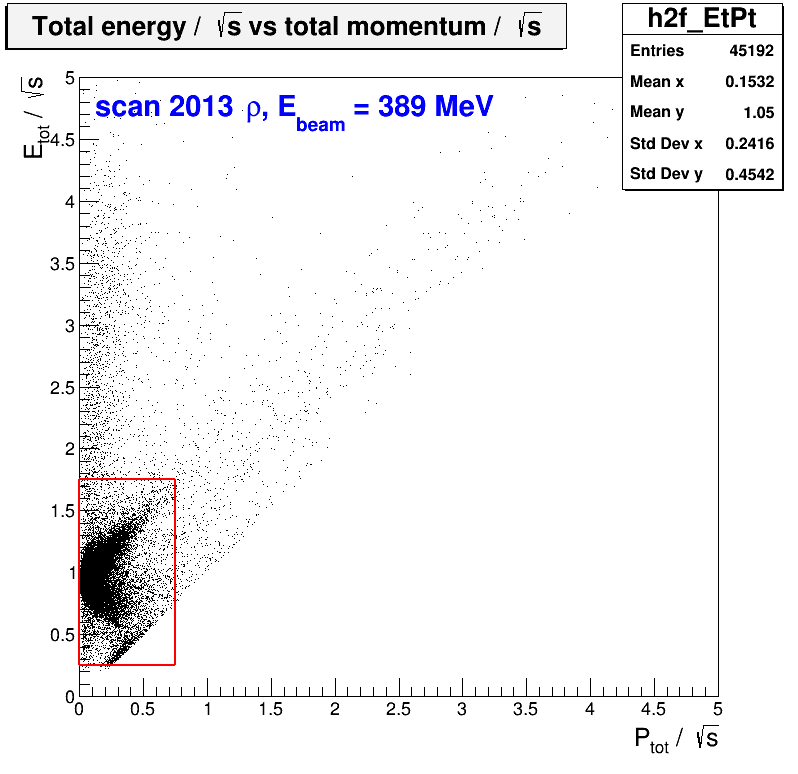
\includegraphics[width=\textwidth]{img/h2f_EtPt.png}
        \caption{Полный вид.}
        \label{fig:EtPt_full}
    \end{subfigure}
    ~
    \begin{subfigure}[b]{0.45\textwidth}
        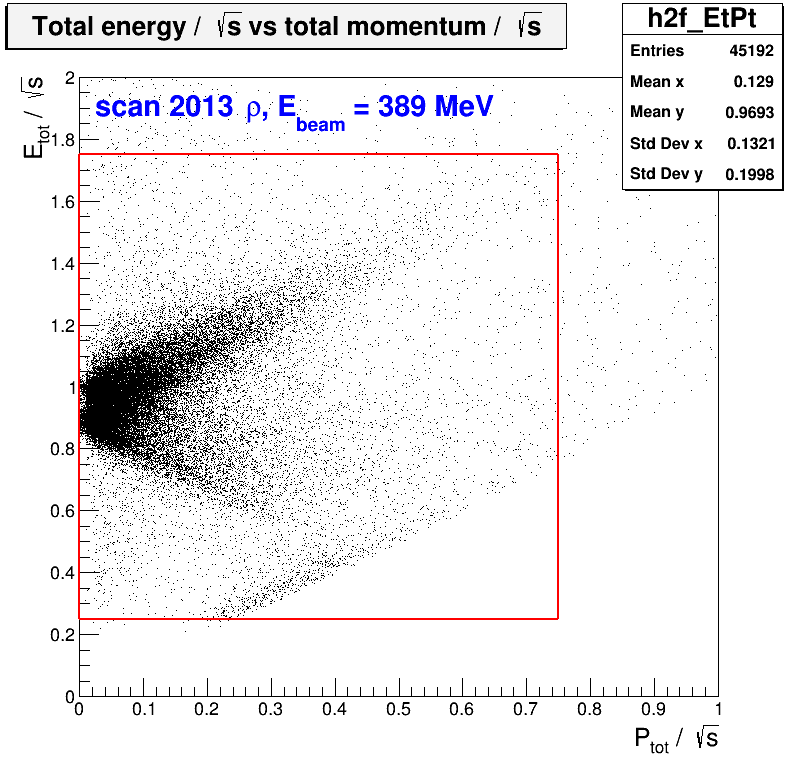
\includegraphics[width=\textwidth]{img/h2f_EtPt_zoom.png}
        \caption{Область выбора приближена.}
        \label{fig:EtPt_zoom}
    \end{subfigure}
    \caption{Распределение полной энергии и полного импульса системы,
        нормированные на $\sqrt{s}$.
        Красной линией обозначены условия отбора.
        Экспериментальные данные сезона $2013 \, \rho$,
        $E_{beam} = \SI{389}{\MeVr}$.}\label{fig:EtPt}
\end{figure}

Для прошедших отборы событий проводится кинематическая реконструкция в гипотезе четырёх частиц (двух заряженных пионов и двух фотонов) с требованием выполнения законов сохранения импульса-энергии для всей системы.
Таким образом после кинематической реконструкции суммарный импульс системы $P^{KF}_{tot}$ стремится к нулю,
а общая энергия системы $E^{KF}_{tot}$ к энергии двух пучков.
\begin{figure}[htbp]
    \centering
    \begin{subfigure}[t]{0.45\textwidth}
        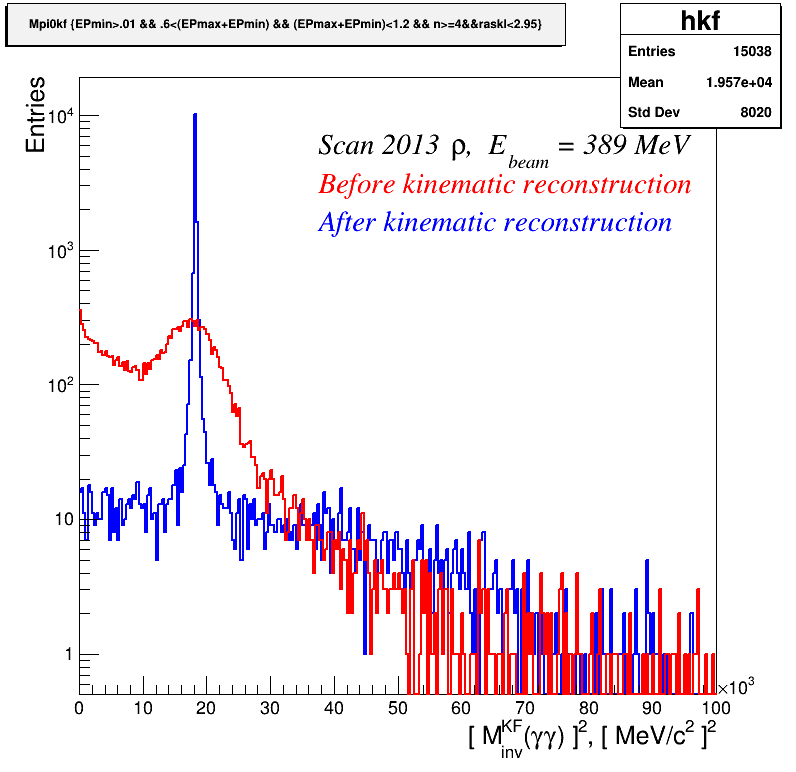
\includegraphics[width=\textwidth]{img/diff_kf_mpi0_2013rho389.png}
        \caption{Данные сезона $2013 \, \rho$, $E_{beam} = \SI{389}{\MeVr}$.}
        \label{fig:diff_kf_mpi0_2013rho389}
    \end{subfigure}
    ~
    \begin{subfigure}[t]{0.45\textwidth}
        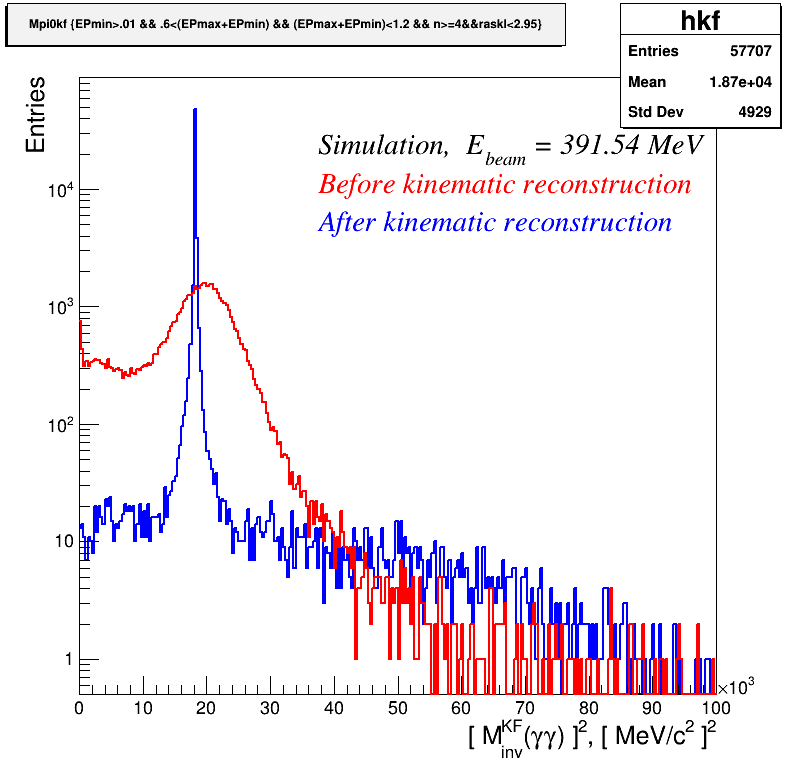
\includegraphics[width=\textwidth]{img/diff_kf_mpi0_sim391_54.png}
        \caption{Моделирование $e^+ e^- \to \pi^+ \pi^- \pi^0$, $E_{beam} = \SI{391.54}{\MeVr}$.}
        \label{fig:diff_kf_mpi0_sim391_54}
    \end{subfigure}
    \caption{Распределение событий по квадрату инвариантной массы двух фотонов для событий с двумя и более фотонами.
    Красная (синяя) гистограмма --- до (после) кинематической реконструкции.}\label{fig:diff_kf_mpi0}
\end{figure}

 
Второй этап отборов начинается с требования на массу отдачи двух заряженных пионов $M_{recoil}^{\pi^+ \pi^-}$,
а именно $\SI{0}{\MeVr} < M_{recoil}^{\pi^+ \pi^-} < \SI{300}{\MeVr}$.
Дополнительно для треков накладывается условие
% $ 0.1 < E_1/p_1 , \, E_2/p_2 < 2 $.
$ E_1/p_1 + E_2 / p_2 < 1$
и $\min(E_i / p_i) > 0.1$.
В то время как на угол между треками $\Omega_{\pi^+ \pi^-}$ накладывается условие $\Omega_{\pi^+ \pi^-} < 2.95$.
Данное условие продемонстрировано на рисунках~\ref{fig:raskl}.
\begin{figure}
    \begin{minipage}[t]{0.45\textwidth}
        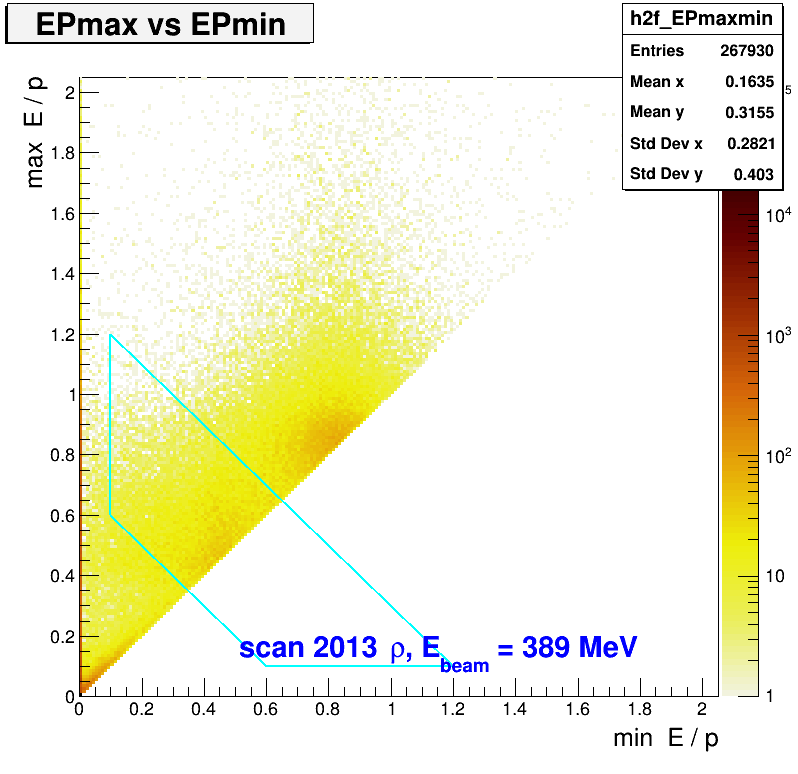
\includegraphics[width=\textwidth]{img/h2f_EPmaxmin_zoom.png}
        \caption{Распределение отношения энерговыделения трека к импульсу трека.
            Голубой линией обозначены условия отбора по $E_i / p_i$.
            Экспериментальные данные сезона $2013 \, \rho$, $E_{beam} = \SI{394}{\MeVr}$.}
        \label{fig:EPmaxmin_zoom}
    \end{minipage}
    \qquad
    \begin{minipage}[t]{0.45\textwidth}
        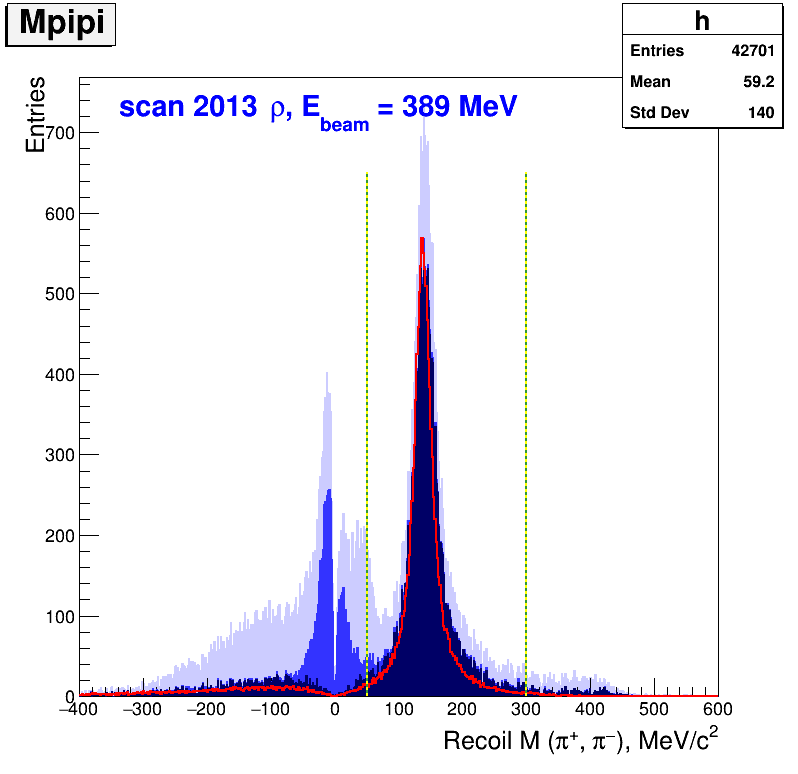
\includegraphics[width=\textwidth]{img/mpipi.png}
        \caption{Тёмно-синяя гистограмма --- с отбором по $E/p$ и $\Omega_{\pi^+ \pi^-}$,
            синяя гистограмма --- с отбором по $E/p$,
            блеклая гистограмма --- до отбора по $E/p$,
            красная линия --- моделирование после отбора по $E/p$ и $\Omega_{\pi^+ \pi^-}$,
            зелёно-жёлтая штрихованная линии --- условия отбора по $M_{recoil}^{\pi^+ \pi^-}$.}
        \label{fig:mpipi}
  \end{minipage}
\end{figure}


\begin{figure}[htbp]
    \centering
    \begin{subfigure}[b]{0.45\textwidth}
        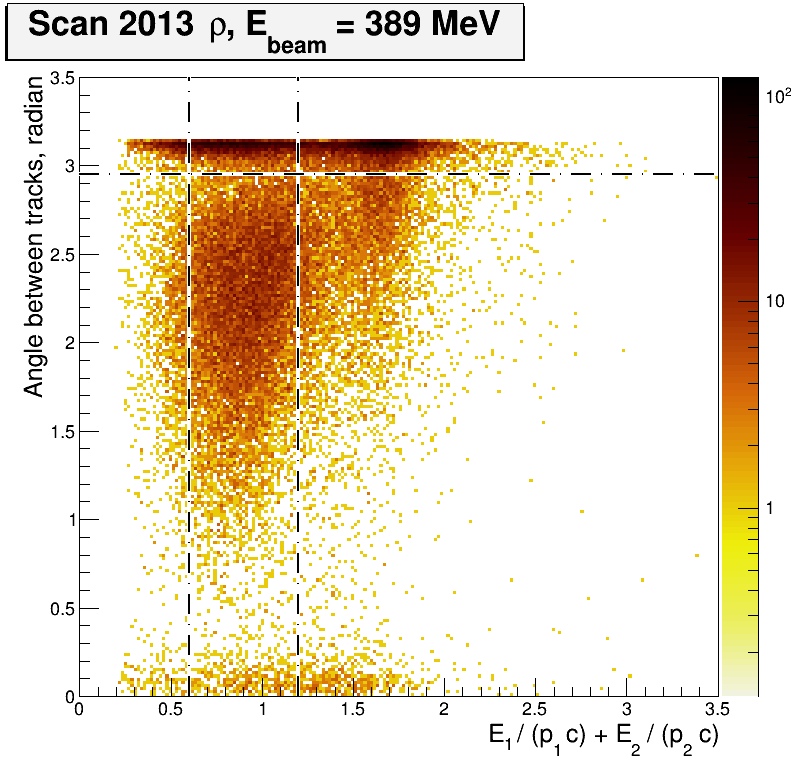
\includegraphics[width=\textwidth]{img/raskl_vs_sumEP_rho389.png}
        \caption{Данные сезона $2013 \, \rho$, $E_{beam} = \SI{389}{\MeVr}$.}
        \label{fig:raskl_rho389}
    \end{subfigure}
    ~
    \begin{subfigure}[b]{0.45\textwidth}
        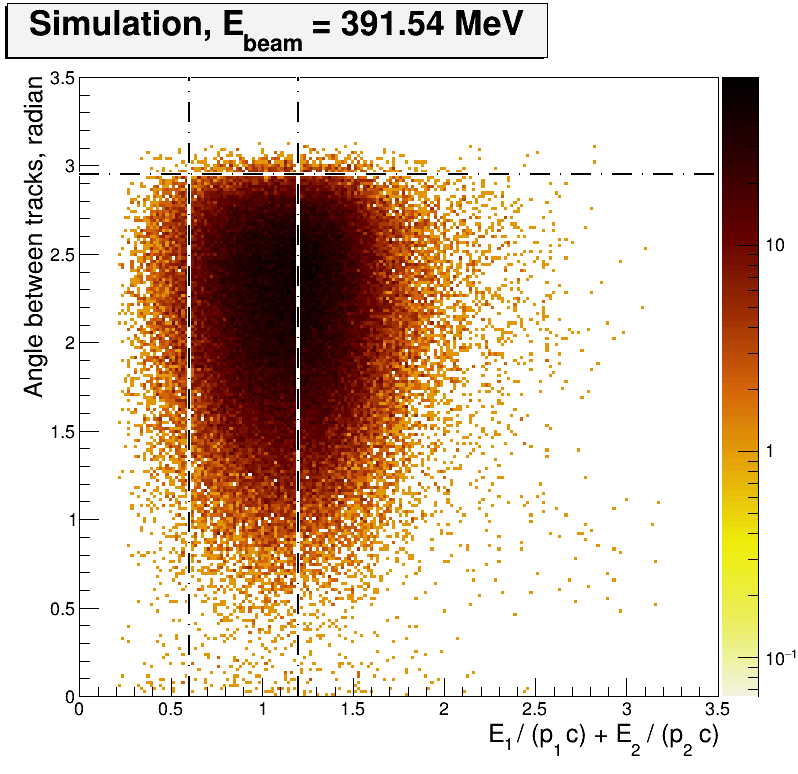
\includegraphics[width=\textwidth]{img/raskl_vs_sumEP_sim391_54.png}
        \caption{Simulation $\pi^+ \pi^- \pi^0$, $E_{beam} = \SI{391.54}{\MeVr}$.}
        \label{fig:raskl_sim391_54}
    \end{subfigure}
    \caption{Distribution of an angle between tracks $\Omega_{\pi^+ \pi^-}$ versus $E_1/p_1 + E_2 / p_2 < 1$.
    Vertical lines represent the used cut on $\sum E_i / p_i$.}\label{fig:raskl}
\end{figure}




\subsubsection{Эффективность триггера}

Вычисление сечений изучаемых реакций требует учёта эффективности нейтрального триггера $\varepsilon_{NT}$,
которая извлекается по событиям радиационного баба рассеяния $e^+e^- \to e^+e^-\gamma$.


Процесс $e^+e^- \to e^+e^-\gamma$ выбран по ряду причин.
Он похож по характеру энерговыделения,
так как и фотоны,
и электроны рождают электромагнитный ливни.
Количество частиц в конечном состоянии равно оному в изучаемых процессах,
а именно трём.
Из первых двух пунктов следует,
что и система нейтрального триггера будет реагировать похожим образом
---
срабатывают те же маски.
В процессе есть как заряженные,
так и нейтральная частицы,
что позволяет использовать две независимые подсистемы запуска детектора,
позволяющие изучать вероятность срабатывания друг друга.
% что позволяет использовать особенности триггера детектора КМД-3
% ---
% две независимых подсистемы запуска детектора.
Сечение процесса $e^+e^- \to e^+e^-\gamma$ плавное и достаточно велико во всей доступной области энергий.


Отбираются события с двумя центральными треками и хотя бы одним фотоном,
при этом на гамма-кванты налагаются дополнительные условия, 
как $0.42 < \theta < \pi - 0.42$, 
так и $E_\gamma > \SI{30}{\MeVr}$.
Центральным треком
---
треком лежащим в том числе в области взаимодействия пучков или рядом с ней
---
считается такой трек,
который удовлетворяет следующим условиям:
\begin{itemize}
	\item максимально расстояние между треком и орбитой пучков не более \SI{6}{\cmr} в плоскоти $\rho-\varphi$;
	\item $\chi^2_{R} < 100$ из подгонки хитов ДК в $\rho$--$\varphi$ плоскости;
	\item $\chi^2_{Z} < 100$ из подгонки хитов ДК в $\rho$--$z$ плоскости.
\end{itemize}
Более того требуется, чтобы хотя бы одна из частиц летела в цилиндрический калориметр:
$ 0.9 < \theta < \pi - 0.9 $.
Последние условие,
как правило,
обеспечивается одним из треков,
ввиду неэффективности восстановления треков при малых полярных углах.

Затем для каждого события вычисляется полная энергия $E_{sys}$ и полный импульс $P_{sys}$ системы частиц,
причём для нейтральных частиц импульс приравнивается к их энергии, а энергия заряженных частиц рассчитывается как $E = \sqrt{p^2 + {m_e}^2}$.
Таким образом последние частицы предполагаются электронами или позитронами с массой $m_e$.
На полный импульс $P_{sys}$ и полную энергию $E_{sys}$ полученной системы частиц накладываются нижеприведённые условия:
\begin{itemize}
    \item $P_{sys} < 0.25 \sqrt{s}$;
    \item $\frac{2}{3} \sqrt{s} + P_{sys} < E_{sys} < 1.25 \sqrt{s}$.
\end{itemize}
Для определения эффективности триггера отбираются события с $\min (E/p) > 0.8$ и $\max (E/p) < 2$.
Такое условие позволяет дополнительно подавить
фон от минимально ионизирующих частиц $\pi^\pm$ и $\mu^\pm$.
при этом происходят два вида отборов с количеством летящих в цилиндрическую часть детектора частиц:
не меньшим одного и не меньше трёх.


Дополнительно для каждого события сохраняется информация о том,
какой из триггеров сработал:
\begin{itemize}
  \item нейтральный триггер;
  \item заряженный триггер;
  \item полный триггер, то есть в событие сработал и заряженный, и нейтральный триггер.
\end{itemize}
Теперь для каждой точки по энергии определяются количества событий, в которых сработал:
\begin{itemize}
  \item только нейтральный триггер --- $N_{NT}$;
  \item только заряженный триггер ---  $N_{CT}$;
  \item полный триггер --- $N_{tot}$.
\end{itemize}
На основе этих данных рассчитывается эффективности нейтрального триггера $\varepsilon_{NT}$,
заряженного триггера $\varepsilon_{CT}$ и полного триггера $\varepsilon_{tot}$.
Пусть произошло $N$ событий $e^+ e^- \to e^+ e^- \gamma$,
тогда можно записать систему уравнений:
\begin{align}
    N_{NT} &= \varepsilon_{NT} \cdot ( 1 - \varepsilon_{CT} ) \cdot N , \\
    N_{CT} &= ( 1 - \varepsilon_{NT} ) \cdot \varepsilon_{CT} \cdot N , \\
    N_{NT} &= \varepsilon_{NT} \cdot \varepsilon_{CT} \cdot N .
\end{align}
Разрешим данные связи относительно искомых эффективностей:
\begin{align}
    \varepsilon_{NT} &= \frac{ N_{tot} }{ N_{tot}+N_{CT} } , \\
    \varepsilon_{CT} &= \frac{ N_{tot} }{ N_{tot}+N_{NT} } , \\
    \varepsilon_{tot} &= 
    \frac{ N_{tot} (N_{tot}+N_{CT}+N_{NT}) }{
        (N_{tot}+N_{CT}) (N_{tot}+N_{NT})
    } \\
    &=
    1 - (1-\varepsilon_{NT}) (1-\varepsilon_{CT}) .
\end{align}
Положив статистическую неопределённость $N_i$,
где $i = NT, \, CT,$ и $tot$,
равными $ \Delta N_i  = \sqrt{N_i} $ можно вычислить погрешности определения эффективностей,
воспользовавшись формулой переноса ошибок.
\[ \Delta  \varepsilon_{NT} = \frac{1}{ ( N_{TC} + N_T )^2} \left[ N_{TC}  N_T ( N_{TC} + N_T )
\right]^\frac{1}{2} \]
\[ \Delta  \varepsilon_{CT} = \frac{1}{ ( N_{TC} + N_C )^2} \left[ N_{TC}  N_C ( N_{TC} + N_C )
\right]^\frac{1}{2} \]
\[ \Delta  \varepsilon_{tot} =  \left[ (1-\varepsilon_{NT})^2 {\Delta  \varepsilon_{CT}}^2 +
(1-\varepsilon_{CT})^2 {\Delta  \varepsilon_{NT}}^2 \right]^\frac{1}{2} \]

Основными фоновыми процессам для $e^+ e^- \to e^+ e^-\gamma$ являются процессы
$e^+ e^- \to \pi^+ \pi^- \gamma$ и $e^+ e^- \to \pi^+ \pi^- \pi^0 \to \pi^+ \pi^- 2\gamma$.
Так как эти процессы носят резонансный характер,
то их вклад в ошибку определения эффективности триггера будет наиболее большим в области $\omega (782)$ и $\phi (1020)$ резонансов.
Для подавление событий с заряженными пионами используется ограничение на отношение импульса частицы,
измеренного трековой системой детектора, к энергии, определённой по данным калориметра.
Для электронов и позитронов это отношение близко к единице.
В случае пионов оно пикуются в области $P/E = \sqrt{1 - {m_{\pi^\pm}}^2 / E^2}$,
так для энергии пиона равной \SI{300}{\MeVr} расчётное $P/E \simeq 0.88$.

Далее определялась эффективность нейтрального триггера,
а также заряженного и полного, в зависимости от диапазона полярных углов частиц.
Будем накладывать ограничение на минимальный угол $\theta_{min}$ между частицами и осью пучков.
Из рисунка \textbf{рисунок} видно,
что начиная с $\theta_{\min} = 0.9$ эффективность стабилизируется и перестаёт зависеть от $\theta_{\min}$,
далее для определения эффективности триггера будет использоваться именно это значение минимального угла.

Теперь определим эффективности триггеров для всей статистики, используемой в данной работе.
На рисунке~\ref{fig:nt_eff} представленность зависимость эффективностей от энергии в системе центра масс.
Видно, что области резонансов наблюдаются некоторые провалы в эффективностях,
наиболее ярко это видно для заряженного триггера.


\begin{figure}
    \centering
    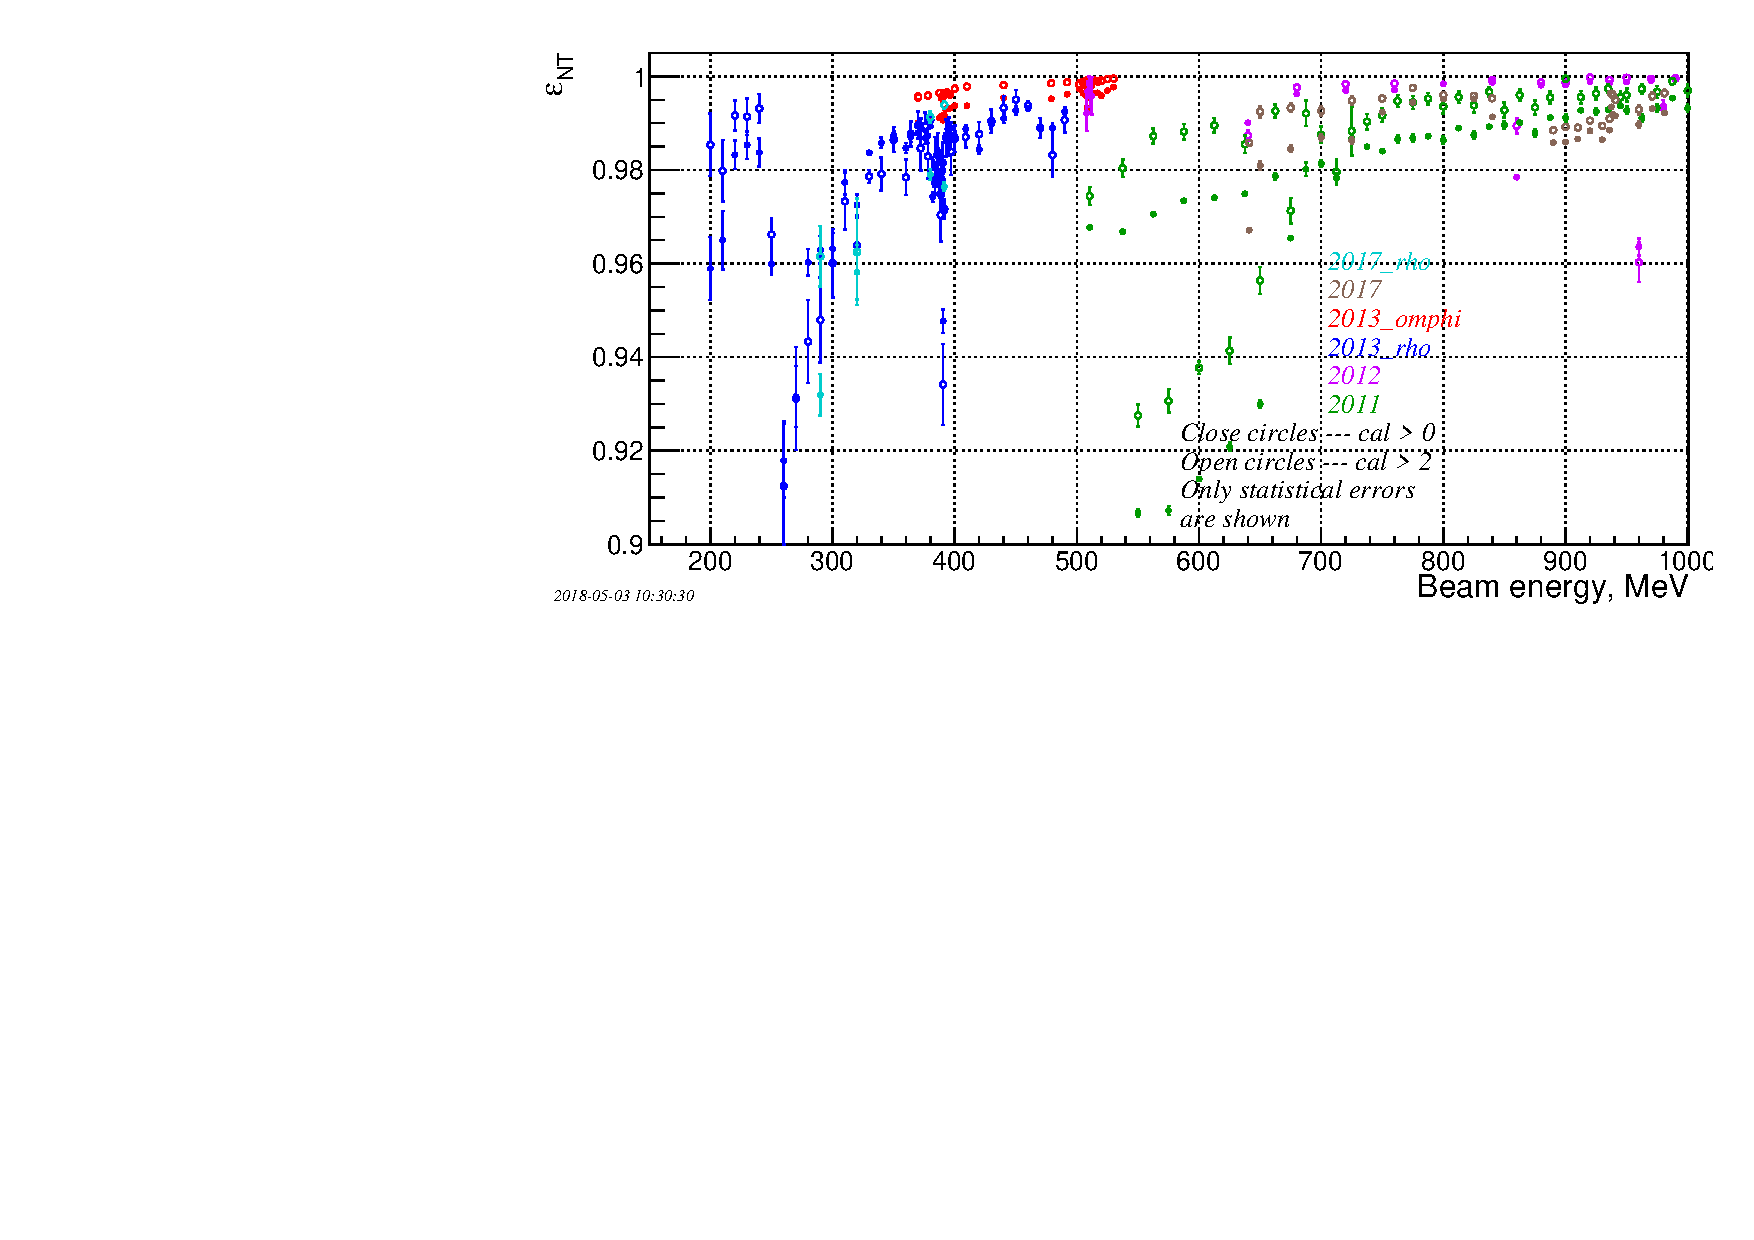
\includegraphics[width=\textwidth]{img/nt_eff.pdf}
    \caption{Эффективность нейтрального триггера.}
    \label{fig:nt_eff}
\end{figure}



% \subsubsection{Учёт радиационных поправок}


% \subsection{Сечение процессов}

Основной задачей данной работы является вычисление сечение реакций
$e^+e^- \to \pi^0 \gamma, \, \eta \gamma$ в доступном диапозоне энергий.
Сечение расчитывается согласно формуле
\begin{equation}
	\sigma = \frac{ N } { L \, (1+\delta_{rad}) \, \varepsilon_{NT} \,
	\varepsilon_{det}} \cdot  
	\left( \frac{ {\varepsilon^{MC}_{\gamma}} }{ {\varepsilon^{exp}_{\gamma}} } \right)^3.
\end{equation}
Здесь $L$ --- интегральная светимость;
$\varepsilon_{det}$ --- эффективность метода, определяется из моделирования;
$\delta_{rad}$ --- радиационная поправка;
$\varepsilon_{NT}$ --- эффективность нейтрального триггера;
вторая дробь соответствует поправке на разницу между моделированием и экспериментом в эффективности
реконструкции фотонов.

Радиационная поправка $\delta_{rad}$ считается по алгоритму, основанному на статье \cite{Kuraev1985}.
Данная поправка является радиационной поправкой к процессам однофотонной аннигиляции $e^+ e^-$-пары,
связанная только с начальным состоянием.
Заявленная точность вычислений не хуже \SI{0.1}{\percent}.
В такую же точность оценивается и вычисление радиационной поправки,
главным образом определяемая алгоритмом аппроксимации сечений интересуемого процесса.
Вычисленные значения $1+\delta_{\text{rad}}$ приведены на рисунке~\ref{fig:rad_corr}.

\begin{figure}[htbp]
	\centering
	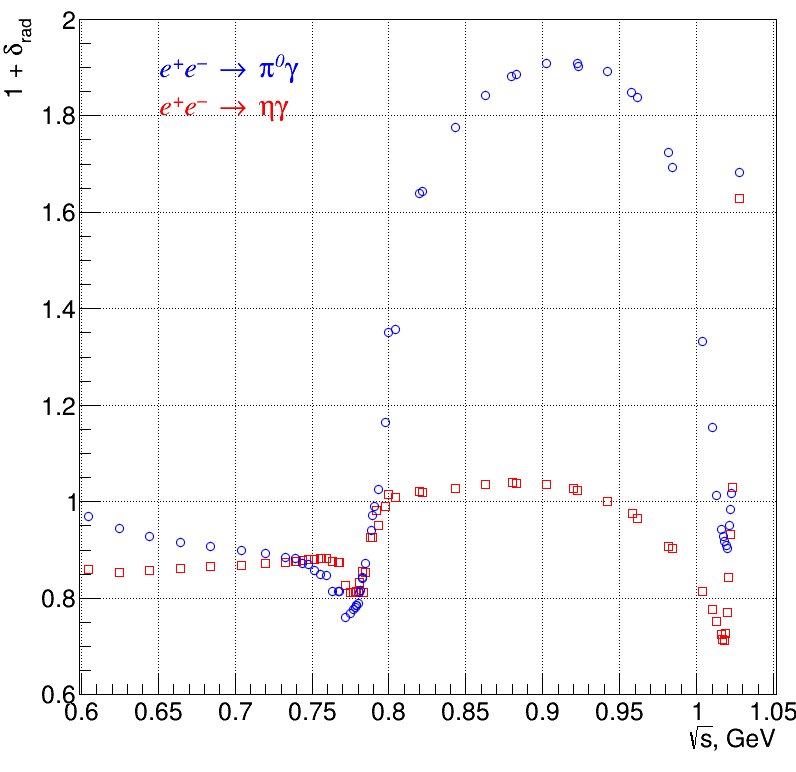
\includegraphics[width=.5\textwidth]{img/rad_corr_for_pseudodisser.png}
	\caption{Радиационная поправка $1+\delta_{\text{rad}}$ для процессов
		$e^+ e^- \to \pi^0 \gamma$ (синие кружки),
		и $e^+ e^- \to \eta \gamma$ (красные квадраты).}\label{fig:rad_corr}
\end{figure}

Инетгральная светимость $L$ на детекторе КМД-3 определяется по процессу Баба рассеяния
$e^+e^- \to e^+e^-$ на большой угол $0.9 < \theta < \pi - 0.9$,
\cite{Ryzhenenkov:2017xqu}.
Достоверность полученных значений контролируется по результатам интгрального сечения $L_{\gamma \gamma}$,
извлекаемого из процесса $e^+e^- \to \gamma \gamma$,
также рассматриваемого в больших углах.
Отличие $1 - L / L_{\gamma \gamma}$ от 0 менее \SI{1}{\percent},
здесь точность ограничено статистикой $e^+e^- \to \gamma \gamma$.

Предварительные результаты по сечения реакций представлены в на рисунках~\ref{fig:cs_pi0g_mine} и~\ref{fig:cs_etag_mine}.

\begin{figure}[htbp]
	\begin{minipage}[T]{.48\textwidth}
		\centering
		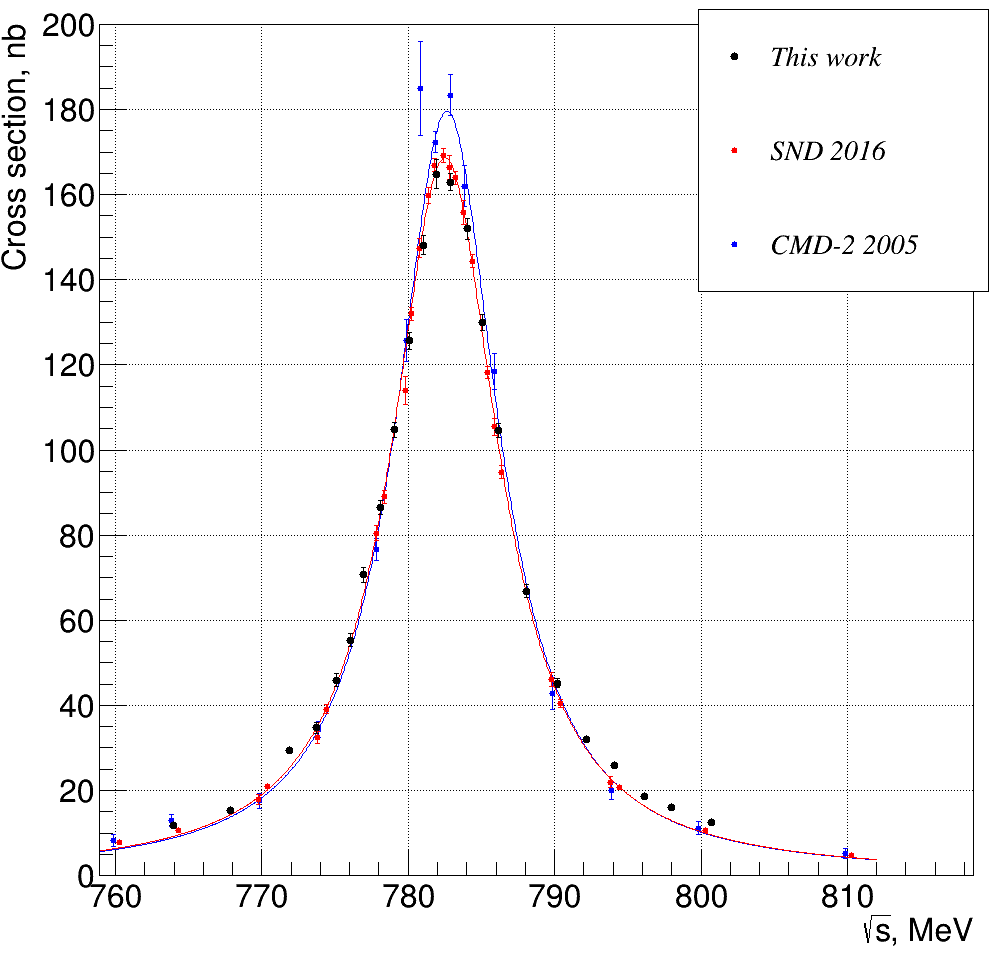
\includegraphics[width=\textwidth]{img/my_pi0g_cross_section_for_pseudodisser.png}
		\caption{Сечение $e^+ e^- \to \pi^0 \gamma$:
			чёрные точки --- предвариетльные результаты данной работы,
			красные (синие) точки и линия --- результаты \cite{Achasov:2016bfr} (\cite{Akhmetshin:2004gw})
			и их аппроксимация нерелятивистк функцией Брейта--Вигнера.}\label{fig:cs_pi0g_mine}
	\end{minipage}
	\begin{minipage}[T]{.48\textwidth}
		\centering
		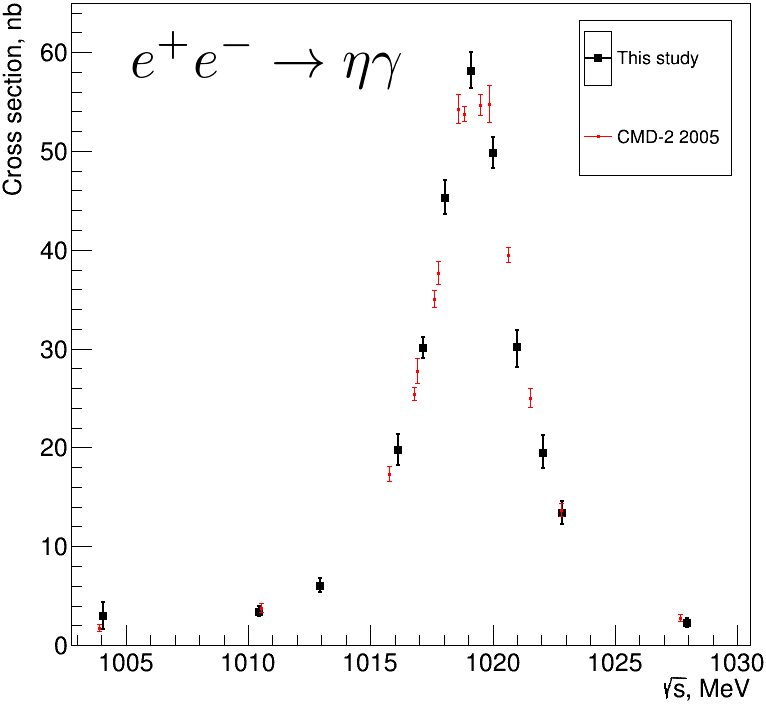
\includegraphics[width=\textwidth]{img/cs_etag_at_phi.png}
		\caption{Сечение $e^+ e^- \to \eta \gamma$:
			чёрные точки --- предвариетльные результаты данной работы,
			красные точки --- результаты \cite{Akhmetshin:2004gw}.}\label{fig:cs_etag_mine}
	\end{minipage}
\end{figure}

%и $e^+e^- \to \gamma \gamma$.%, \cite{lumAkhmetshin2012b}.
%Такой подход позволяет лучше понять и оценить систематические ошибки, которое находятся на уровне \SI{\sim2}{\percent}.
%В ходе определения светимости используются данные моделирования,
%полученные с помощью Монте-Карло генератора фотонных струй (Monte-Carlo Generator Photon Jets)%, \cite{Arbuzov2006}, \cite{Actis2010}),
%модефицированного для изучения продуктов реакций  $e^+e^- \to e^+e^-, \gamma \gamma$.
%Точность расчёта этих сечений с учётом радиационных поправок лучше, чем \SI{0.2}{\percent}.

%Для сравнения полученных сечений с мировыми данными исользованны результаты работ ... .
%Так как данные для процесса $e^+ e^- \to \eta \gamma$ приведенны для различных мод распада $\eta$-мезона,
%то для перевода сечений к одной шкале используются данные %\cite{Beringer:1900zz}.

% \subsubsection{Аппроксимация сечения}

\newpage
\section{Заключение}


В течении всего периода работы детектора КМД -3 систематически проводились калибровки и ремонтное обслуживание электроники катодного тракта Z-камеры.
Разработан алгоритм нахождения и восстановления продольной координаты кластера по катодным полоскам Z-камеры. 
Этот алгоритм добавлен в модуль реконструкции кластера Z-камеры. 
На событиях Баба рассеяния получено пространственное разрешение \~500 мкм.
Разработан алгоритм отделения треков, принадлежащих каонам и пионам, от других треков.
Отлажен алгоритм разделения каонов от пионов в четырёх-трековых и трёх-трековых событиях для процесса .
Определен набор условий для отбора событий этого процесса.
С использованием моделирования по фазовому объему вычислена эффективность регистрации. Построено сечение процесса .
Выделены четыре промежуточных состояния процесса .
Для улучшения точности восстановления импульса трека в программ у добавлен кинематический фит.
В заключение хотелось бы выразить благодарность Г.В. Федотовичу, Е.П. Солодову, А.С. Попову, И.Б. Логашенко, Б.И. Хазин у за полезные советы и помощь.
А тек же, я хочу поблагодарить весь коллектив детектора КМД-3 и комплекса ВЭПП-2000 за их огромный вклад в эксперимент.

% \section{Заключение}

% Список упомянутых тем уже не мал, да может быть ещё расширен.
% В целом измерение сечения процессов $e^+e^- \to \eta \gamma$ и $e^+e^- \to \pi^0 \gamma$ представляются интересной задачей, определённо имеющая своё место в физике высоких энергий.

\newpage
% \bibliographystyle{plain}
\printbibliography

% \bibliography{sample}

\end{document}


